\documentclass[ngerman,UKenglish]{scrbook}
%------------------------------------------------------------------------------
% This file contains a skeleton thesis for
% a Physics or Astronomy Institute in the University of Bonn
%
% Specify the language(s) in the class and then use babel.
% If you need more than one language, give the default language last,
% e.g. ngerman,UKenglish for a thesis in British (UK) English where you want
% to be able to set the language to German for some part of it.

%------------------------------------------------------------------------------
% Set to 2009 for biblatex and bibtex8 (TeX Live 2009)
% Set to 2011 for biblatex and biber   (TeX Live 2011 or later)
% This must be set before \usepackage{ubonn-thesis}
\newcommand*{\texlive}{2011}

%------------------------------------------------------------------------------
\usepackage{ubonn-thesis}
% Glossary package
% \usepackage[acronym,toc]{glossaries}
% TikZ packages and libraries
% \usepackage{tikz}
% \usepackage{tikz-3dplot}
% \usepackage{pgfplots}
% \usetikzlibrary{positioning,shapes,arrows}
% \usetikzlibrary{decorations.pathmorphing}
% \usetikzlibrary{decorations.markings}
\usepackage{thesis_defs}

%------------------------------------------------------------------------------
% Instead of colouring  links, cites, table of contents etc.
% put them in a coloured box for the screen version.
% This is probably a good idea when you print your thesis.
% \hypersetup{colorlinks=false,
%   linkbordercolor=blue,citebordercolor=magenta,urlbordercolor=darkgreen
% }

%------------------------------------------------------------------------------
% When writing your thesis it is often helpful to have the date and
% time in the output file. Comment this out for the final version.
%
\ifoot[\today{} \thistime]{\today{} \thistime}

% Include the words DRAFT on the cover pages - turned off for \mainmatter
% Comment this out before you submit!
% \usepackage{background}
% \backgroundsetup{contents=DRAFT, color=blue!30}

% In order to check if your labels are referenced try the refcheck package
% \usepackage{refcheck}

%------------------------------------------------------------------------------
% Use bibtex8 for TeX Live 2009
%   If you do not have umlauts etc. in your refs, you can drop bibencoding=latin1
% Use biber   for TeX Live 2011 or later
% Add option backref=true to also find out where citations are
% referred to.
\ifthenelse {\texlive = 2009} {%
  \usepackage[backend=bibtex8,hyperref=true,bibencoding=latin1,
    style=numeric-comp,sorting=none,block=ragged,firstinits=true]{biblatex}
}{%
  \usepackage[backend=biber,
    style=numeric-comp,sorting=none,block=ragged,firstinits=true]{biblatex}
}
% Specify the bibliography files here and not at the end!
% Use standard_refs-bibtex if you use bibtex8
% and standard_refs-biber  if you use biber
\ifthenelse {\texlive = 2009} {%
  % Adjustments to output are in this style file:
  \usepackage{../biblatex/biblatex-num-v2009}
  \bibliography{thesis_refs.bib,%
    ../refs/standard_refs-bibtex.bib}
}{%
  % Adjustments to output are in this style file:
  \usepackage{../biblatex/biblatex-num-v2011}
  \addbibresource{thesis_refs.bib}
  \addbibresource{../refs/standard_refs-biber.bib}
}
%
% You can include the following lines if you want to shorten your
% bibliography by not including url fields
% \AtEveryBibitem{\clearfield{url}}
% \AtEveryCitekey{\clearfield{url}}

%------------------------------------------------------------------------------
% The following definitions are used to produce the title pages
% needed at various stages
\newcommand{\thesistitle}{Title of the Thesis}
\newcommand*{\thesisauthor}{Author's name}
\newcommand*{\thesistown}{Place of birth}
\renewcommand*{\InstituteName}{\PI}
\renewcommand*{\inInstitute}{\inPI}
\renewcommand*{\InstituteAddress}{\PIaddress}
% Adjust \thesisreferee...text depending on male/female referee
\newcommand*{\thesisrefereeonetext}{1.\ Gutachter}
\newcommand*{\thesisrefereeone}{Prof.\ Dr.\ John Smith}
\newcommand*{\thesisrefereetwotext}{2.\ Gutachterin}
\newcommand*{\thesisrefereetwo}{Prof.\ Dr.\ Anne Jones}
% Date when thesis was submitted (Master/Diplom)
% Year or Month, Year when thesis was submitted (PhD)
\newcommand*{\thesissubmit}{XX.YY.2013}
% \newcommand*{\thesissubmit}{Month 2013}
% Date of thesis examination (PhD)
\newcommand*{\thesispromotion}{XX.YY.2013}
% Month and year of the final printed version of the thesis
\newcommand*{\thesismonth}{MMM}
\newcommand*{\thesisyear}{2013}
\newcommand*{\thesisnumber}{BONN-IR-2013-XXX}

%------------------------------------------------------------------------------
% The abstract is only needed for the printed version and should be in
% English regardless of the language of the thesis
\newcommand{\thesisabstract}{%
  \begin{otherlanguage}{UKenglish}
    This is your thesis abstract. It may be in a language that is
    different from the rest of your thesis.
  \end{otherlanguage}
}

%------------------------------------------------------------------------------
% \includeonly can be used to select which chapters you want to process
% A simple \include command just inserts a \clearpage before and after the file
% Note that \includeonly can be quite picky! Do not forget to put a
% comma after the filename, otherwise it will simply be ignored!
% \includeonly{%
%   thesis_intro,
%   thesis_appendix,
%   thesis_acknowledge
% }

%------------------------------------------------------------------------------
% Give a list of directories where figures can be found. Do not leave
% any spaces in the list and end the directory name with a /
\graphicspath{%
  {../figs/},%
  {../figs/cover/},%
  {../figs/graphics/},%
  {../feynmf/}%
}

%------------------------------------------------------------------------------
% Make a glossary and a list of acronyms
% \makeglossaries

% Glossary entries
% \input{thesis_glossary}

%------------------------------------------------------------------------------
\begin{document}

% Cover page of thesis - this is only needed for the printed final
% version to be submitted to the department library
% Do not use this page for thesis submission to the Prüfungsamt or Promotionsbüro!
% \input{../cover/PhD_Cover}
% \input{../cover/Master_Cover}
% \input{../cover/Diplom_Cover}

% Start counting pages from the title page
\frontmatter
% Dedication has to come before \maketitle
% \dedication{For ...}

%------------------------------------------------------------------------------
% PhD Title page
% Use this command when you submit your thesis
% \input{../cover/PhD_Submit_Title}
% Use this command for the print version
% \input{../cover/PhD_Final_Title}

%------------------------------------------------------------------------------
% Diplom Title page
% Use this command when you submit your thesis
% \input{../cover/Diplom_Submit_Title}
% Use this command for the print version
% \input{../cover/Diplom_Final_Title}

%------------------------------------------------------------------------------
% Master Title page
% Use this command when you submit your thesis
\input{../cover/Master_Submit_Title}
% Use this command for the print version
% \input{../cover/Master_Final_Title}

%------------------------------------------------------------------------------
% Bachelor Title page
% \input{../cover/Bachelor_Title}

\pagestyle{scrplain}

%------------------------------------------------------------------------------
% You can add your acknowledgements here - don't forget to also add
% them to \includeonly above
%------------------------------------------------------------------------------
\chapter*{Danksagung}
\label{sec:ack}
%------------------------------------------------------------------------------

\begin{otherlanguage}{ngerman}
Und das war es jetzt\dots\ Fehlt nur noch ein ganz gro\ss{}es Dankesch\"on an 
alle, ohne die diese Arbeit so nicht m\"oglich und die Zeit nicht so sch\"on 
gewesen w\"are.

Zuerst nat\"urlich an Marek Kowalski, der mir schon fr\"uh die Promotionsstelle 
zugesagt und mir sogar -- lang, lang ists her -- zu meiner Diplomarbeit schon 
ein paar n\"utzliche Tips gegeben hat. Auch sp\"ater war trotz vollen 
Terminplans und am Schluss auch gro\ss{}er Entfernung (fast) immer Zeit f\"ur 
ein paar hilfreiche Worte.
Danke auch an Norbert Wermes f\"ur die \"Ubernahme der Zweitkorrektur.

Dann der Bonner Doppel-Arbeitskreis. Sehr spannende Konstruktion, zwei doch 
ziemlich unterschiedliche Themen unter einem Dach. Erst mal vielen Dank an alle 
f\"ur die sch\"one Arbeitsatmosph\"are, den vielen leckeren Kuchen und die 
allmitt\"agliche Tee- und Kaffeepause. Besonderen Dank an meine flei\ss{}igen 
Korrekturleser Andreas, Markus, Alex und Marcel. Und weil Ruth auch was gelesen 
hat, sind meine Erg\"usse hoffentlich auch f\"ur Nicht-IceCuber verst\"andlich. 

Sebastian hat zwar nichts gelesen, aber trotzdem wohl am meisten beigetragen. 
Ob beim Programmieren, Debuggen, bei der Analyse oder bei Pr\"asentationen: 
Immer gab es hilfreiche Kommentare und Anregungen. Unter denen mag ich manchmal 
auch etwas gest\"ohnt haben, aber ein Faultier wie ich braucht den 
gelegentlichen Tritt in den Hintern. Und zur Belohnung ist er ja jetzt Prof 
im goldische Meenz.

Womit wir auch schon bei der Family w\"aren. Allen voran meine Schwestern 
Judith und Johanna, die zwar mittlerweile schon richtig erwachsen, aber 
trotzdem noch die lustigsten und liebsten Schwestern sind, die man haben kann. 
Au\ss{}erdem k\"onnen sie mich vermutlich beide unter den Tisch trinken -- 
Studenten halt. Dazu mein Onkel Mani, der tats\"achlich fast gleichzeitig mit 
mir aus Mainz gen Norden gezogen ist, allerdings nicht ganz so weit. Und meine 
Eltern: Danke f\"ur alles, trotz Allem.

Und zum Schluss noch einmal nach Bonn, zu den Polyphonikern: Ein toller Chor, 
nicht nur musikalisch, mit dem ich mich hier direkt heimisch gef\"uhlt habe. 
Dort hinzugehen, war eine der, wenn nicht die beste und wichtigste Entscheidung 
meines Lebens. 

Denn jetzt habe ich die beste Michi der Welt. Du hast mir das verr\"uckteste 
und sch\"onste Jahr meines Lebens geschenkt, dem noch bessere folgen werden. 
Und den besten Grund \"uberhaupt, endlich mal fertig zu werden. 

Das bin ich hiermit.


\end{otherlanguage}

%%% Local Variables: 
%%% mode: latex
%%% TeX-master: "../mythesis"
%%% End: 


\tableofcontents

\mainmatter
\pagestyle{scrheadings}

% Turn off DRAFT for the following pages
% \backgroundsetup{contents={}}

%------------------------------------------------------------------------------
% Add your chapters here - don't forget to also add them
% to \includeonly above
%==============================================================================
\chapter{Introduction}
\label{sec:intro}
%==============================================================================

Although the first conclusive observation of neutrino oscillations was made not
even twenty years ago, this phenomenon of neutrinos changing their flavour when
travelling macroscopic distances has been one of the major areas of research in
particle physics and astrophysics ever since. Up to now, it is the only
manifestation of so-called ``physics beyond the standard model'' that has been
confirmed experimentally. During the past two decades, many dedicated
experiments have mapped out the parameters characterising neutrino oscillations
in great detail, leaving only two parameters to be determined.

One of these parameters is the so-called neutrino mass hierarchy. It refers to
the sign of another parameter, one of the two independent mass splittings,
whose absolute value has already been measured.

%------------------------------------------------------------------------------
\appendix
% \part*{Appendix}
%
% Add your appendices here - don't forget to also add them
% to \includeonly above
\chapter{Applicability of the Fisher Matrix}
\label{app:fisher_valid}

As established in Sec.~\ref{sec:fisher_prereq}, one requirement for the Fisher
Matrix to be valid is that the observables (\ie the bin counts for PINGU) are
described by linear functions of the parameters, hence the partial derivatives
entering (\ref{eqn:fisher_def}) can be considered to be constant within the
considered range. To quantify the non-linearity, one can define the quantity
\begin{equation}
 \Upsilon_n(p_i) = \left(N_n(p_{i,\,\mathrm{fid}} + \sigma_{p_i}) -
                          N_n(p_{i,\,\mathrm{fid}}) +
                     \frac{\partial N_n}{\partial p_i}\sigma_{p_i}\right)
                       \bigg/ N_n(p_{i,\,\mathrm{fid}}) \quad,
 \label{eqn:non-lin}
\end{equation}
describing the relative contribution of the non-linear terms to the variation
of the event count $N_b$ in bin $b$ as a function of the parameter $p_i$ over
its uncertainty range $p_{i,\,\mathrm{fid}} \pm \sigma_{p_i}$.

As one can see from Figs.~\ref{fig:nonlinearities1} and
\ref{fig:nonlinearities2}, for the simple scaling parameters like the mass
hierarchy $h$ or the overall normalisation $n_\aeff$ non-linearities are on the
order of the machine precision. But also for the physics parameters they are
typically smaller than $10^{-3}$, hence the requirement of linearity is well
fulfilled.

For means of illustration, the actual dependence of all bin entries on the
systematic parameters is shown as well. By eye, deviations from linearity can
only be recognised for \dm{31} and the energy scale. Since both shift the
sinusoidal oscillation pattern in energy non-linearities have to be expected,
however they only occur on a scale conceivably larger than the actual
uncertainty range.

\begin{figure}[p]
 \centering
 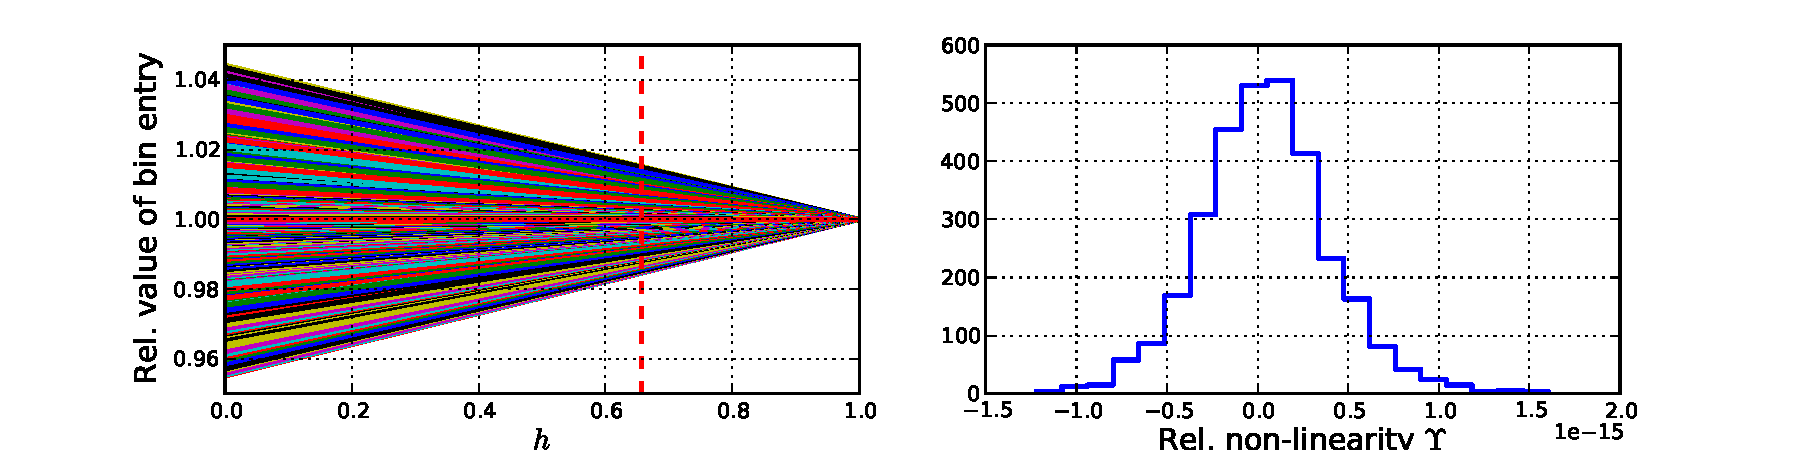
\includegraphics[width=\linewidth]{hierarchy}
 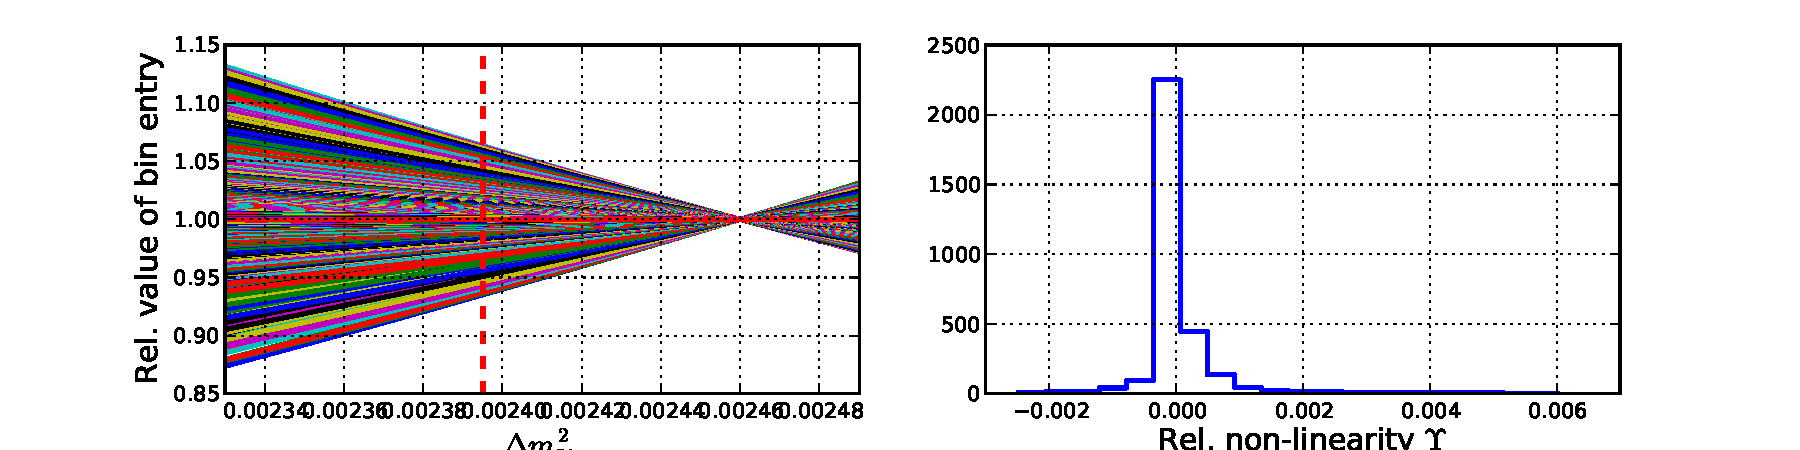
\includegraphics[width=\linewidth]{deltam31}
 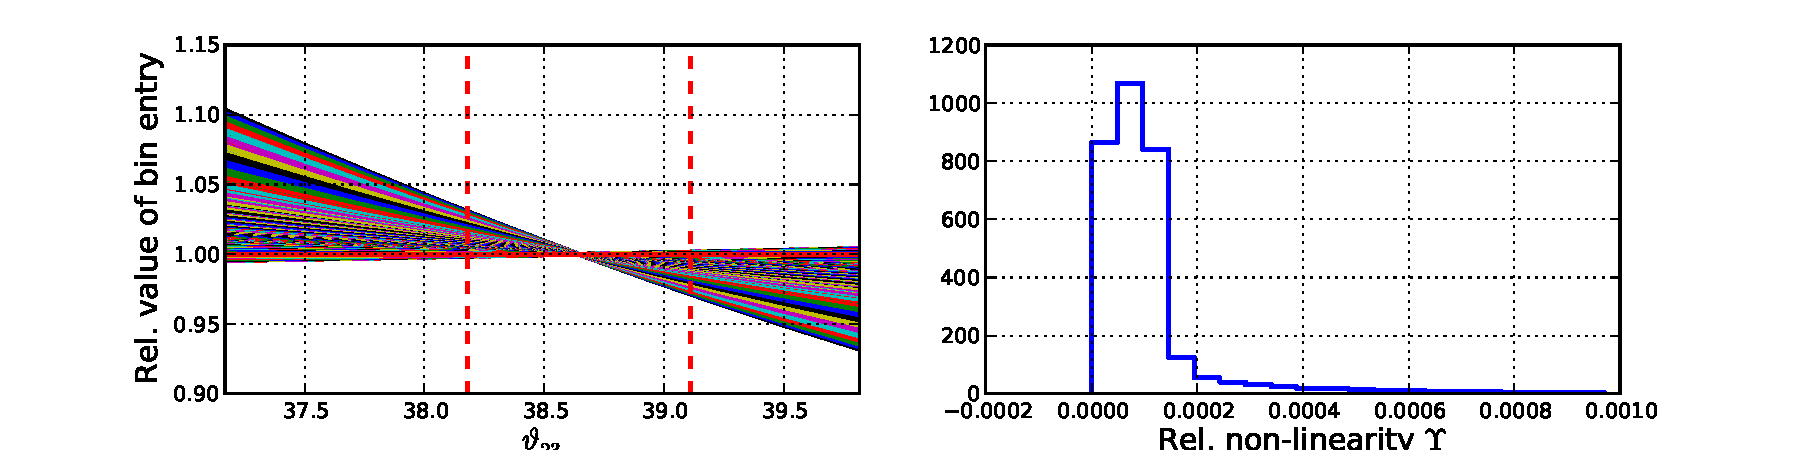
\includegraphics[width=\linewidth]{theta23}
 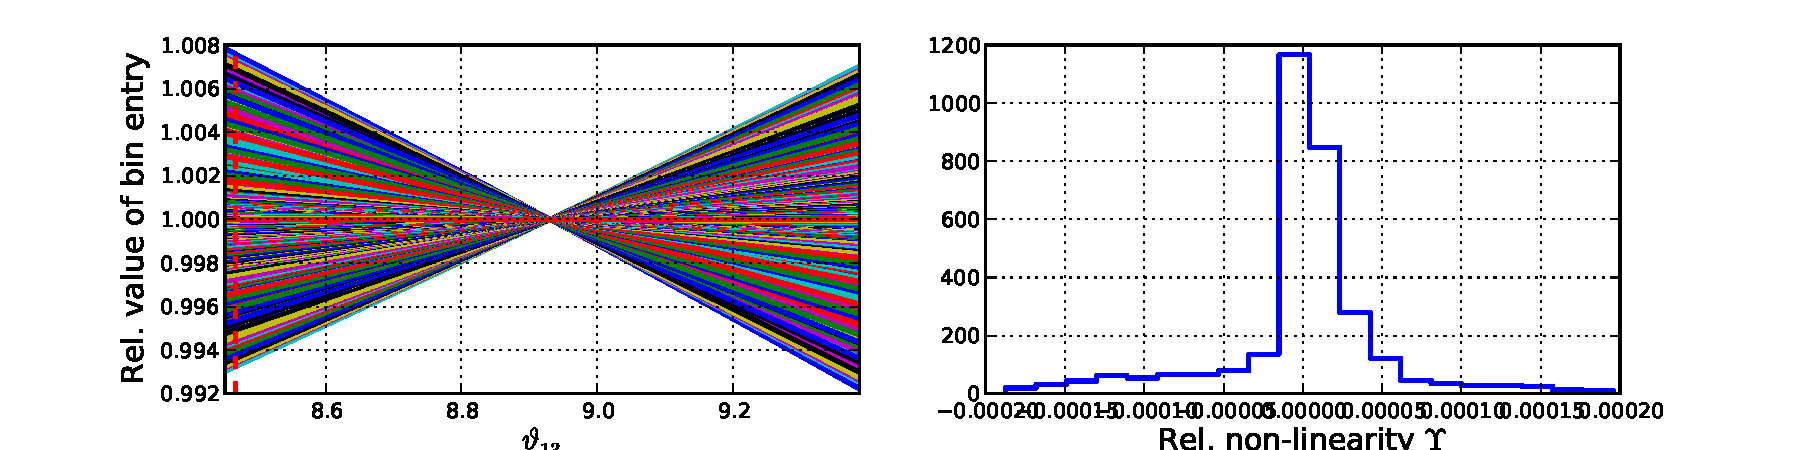
\includegraphics[width=\linewidth]{theta13}
 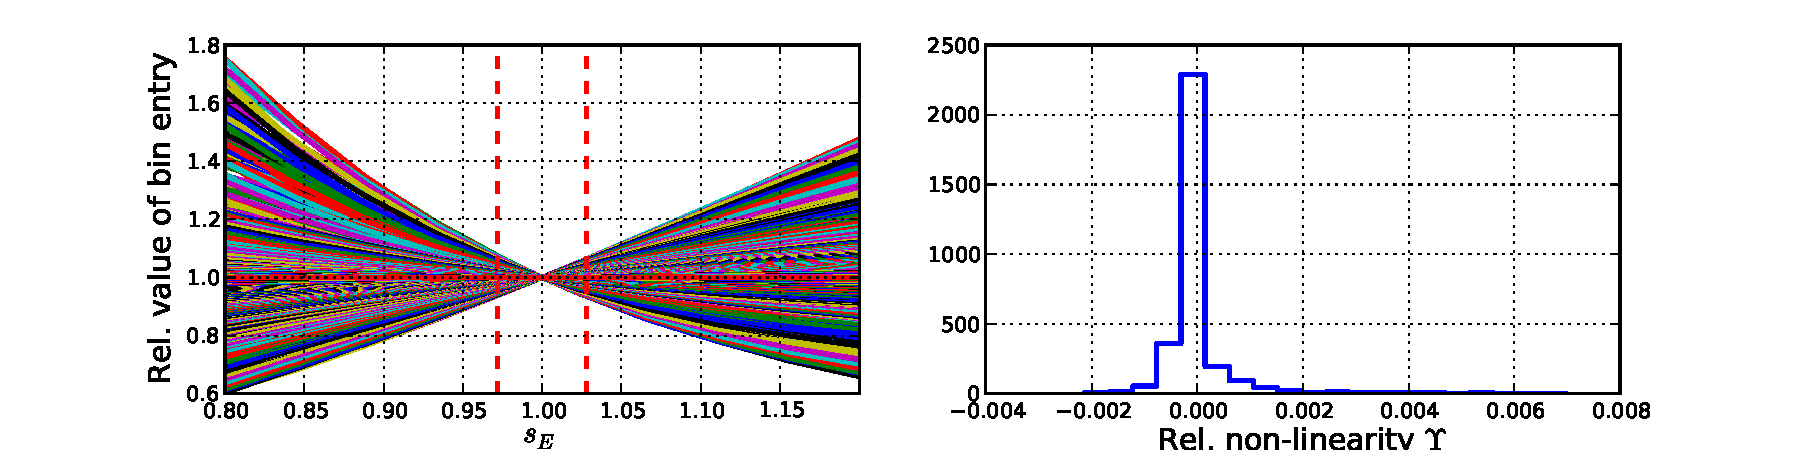
\includegraphics[width=\linewidth]{energy_scale}
 \caption{\emph{Left:} Relative values of all bin entries in the analysis
  histograms as functions of the systematic parameters. The the entries at the 
  fiducial parameter values are set to one. The vertical lines indicate the full
  error range as listed in Tab.~\ref{tab:baseline_results}. \\
  \emph{Right:} Histograms of the non-linearities $\Upsilon$ of the bin counts
  as functions of different systematic parameters (see equation
  (\ref{eqn:non-lin})).}
 \label{fig:nonlinearities1}
\end{figure}

\begin{figure}[p]
 \centering
 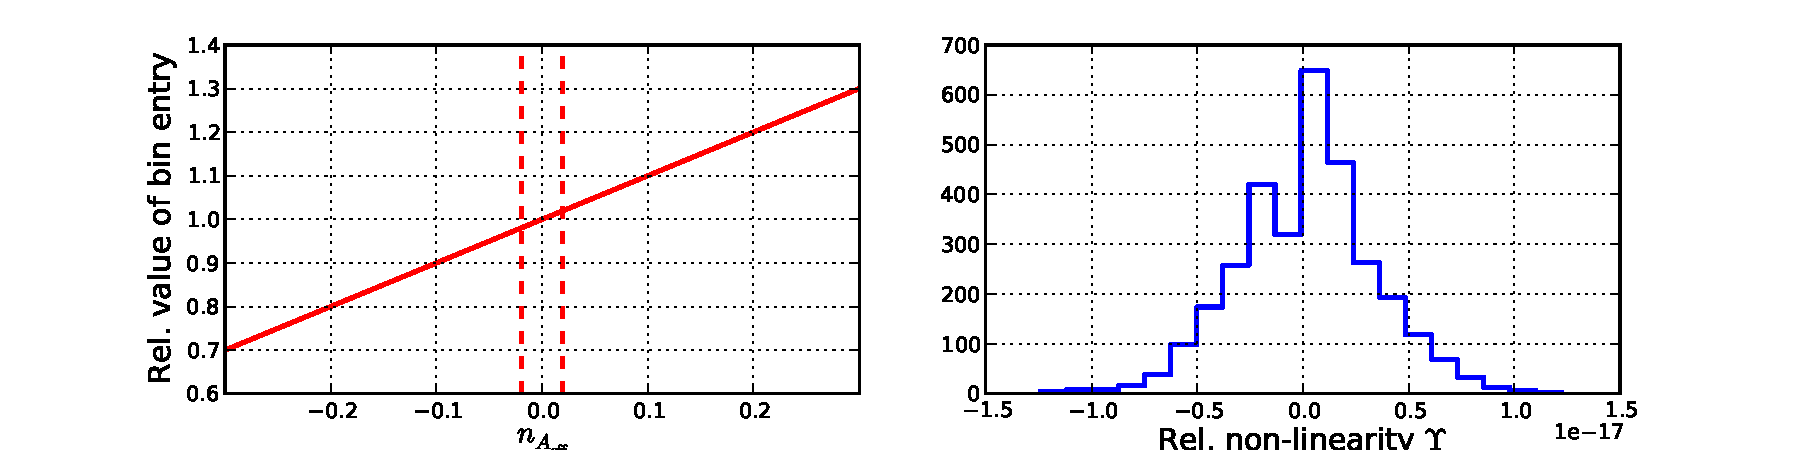
\includegraphics[width=\linewidth]{a_eff_scale_flat}
 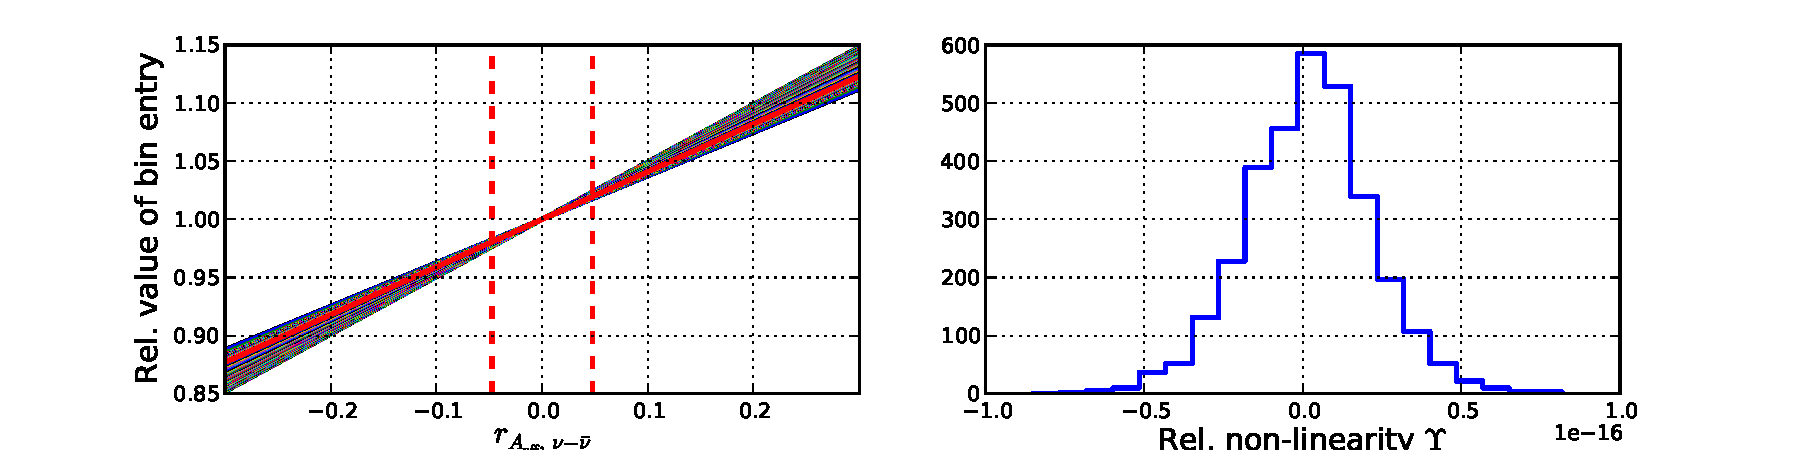
\includegraphics[width=\linewidth]{nu_rel_xsec_scale}
 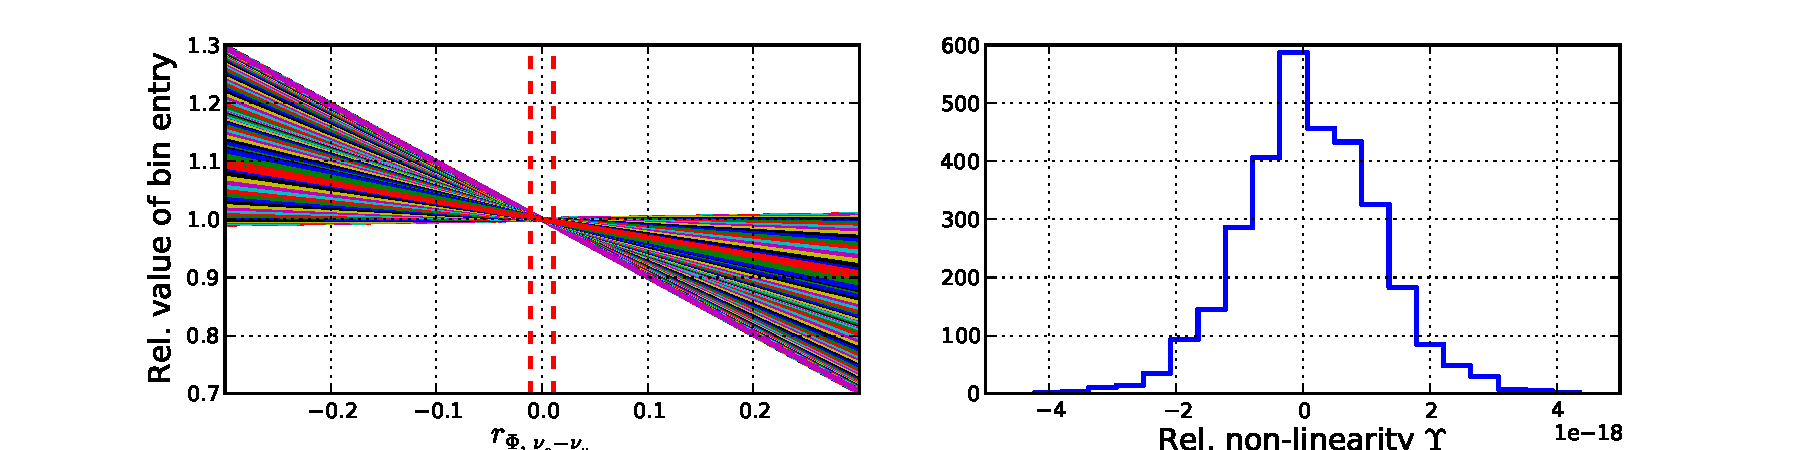
\includegraphics[width=\linewidth]{nue_numu_flux_scale}
 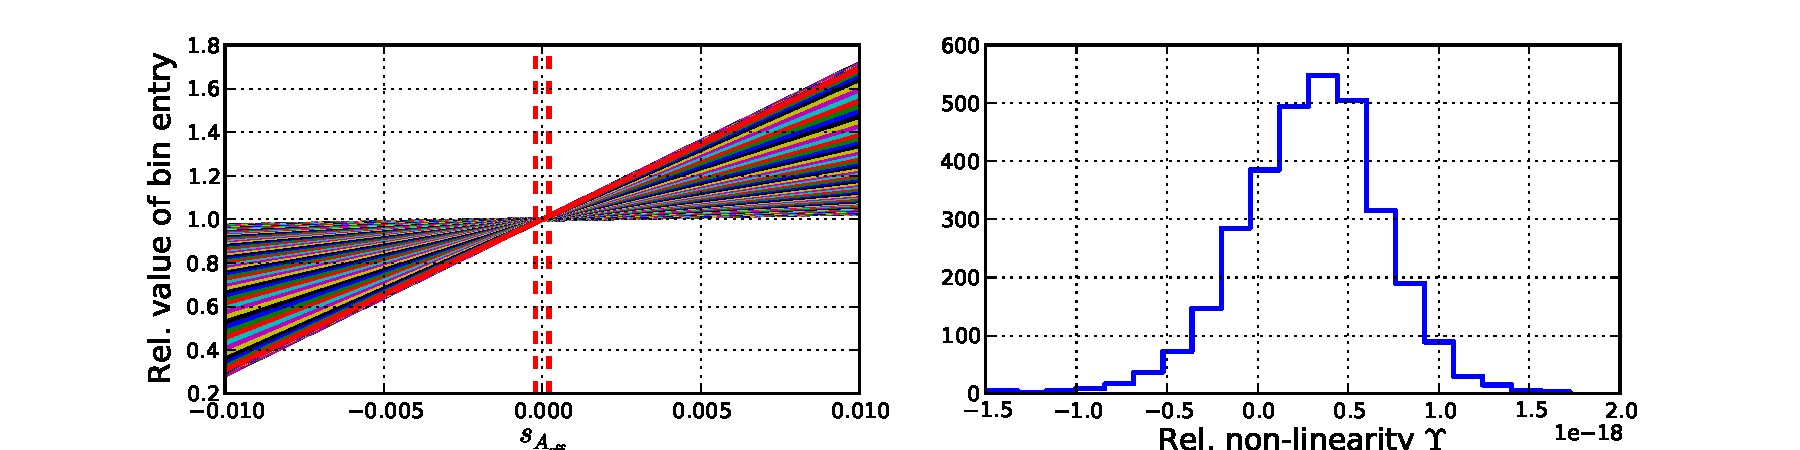
\includegraphics[width=\linewidth]{a_eff_scale}
 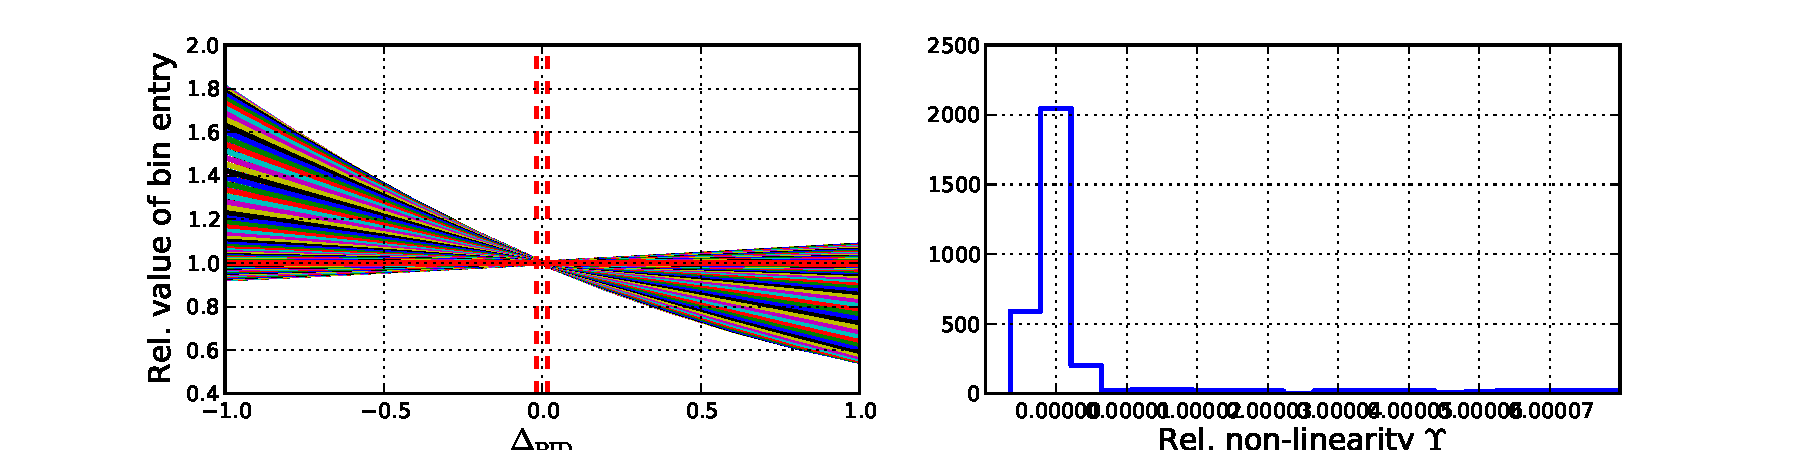
\includegraphics[width=\linewidth]{PID_offset}
 \caption{Same as Fig.~\ref{fig:nonlinearities1} for the remaining parameters.}
 \label{fig:nonlinearities2}
\end{figure}


\chapter{Oscillation Probabilities}
\label{app:oscillation}

\section*{\refstepcounter{section}\thesection\quad Baseline Settings}

\begin{figure}[h]
 \centering
 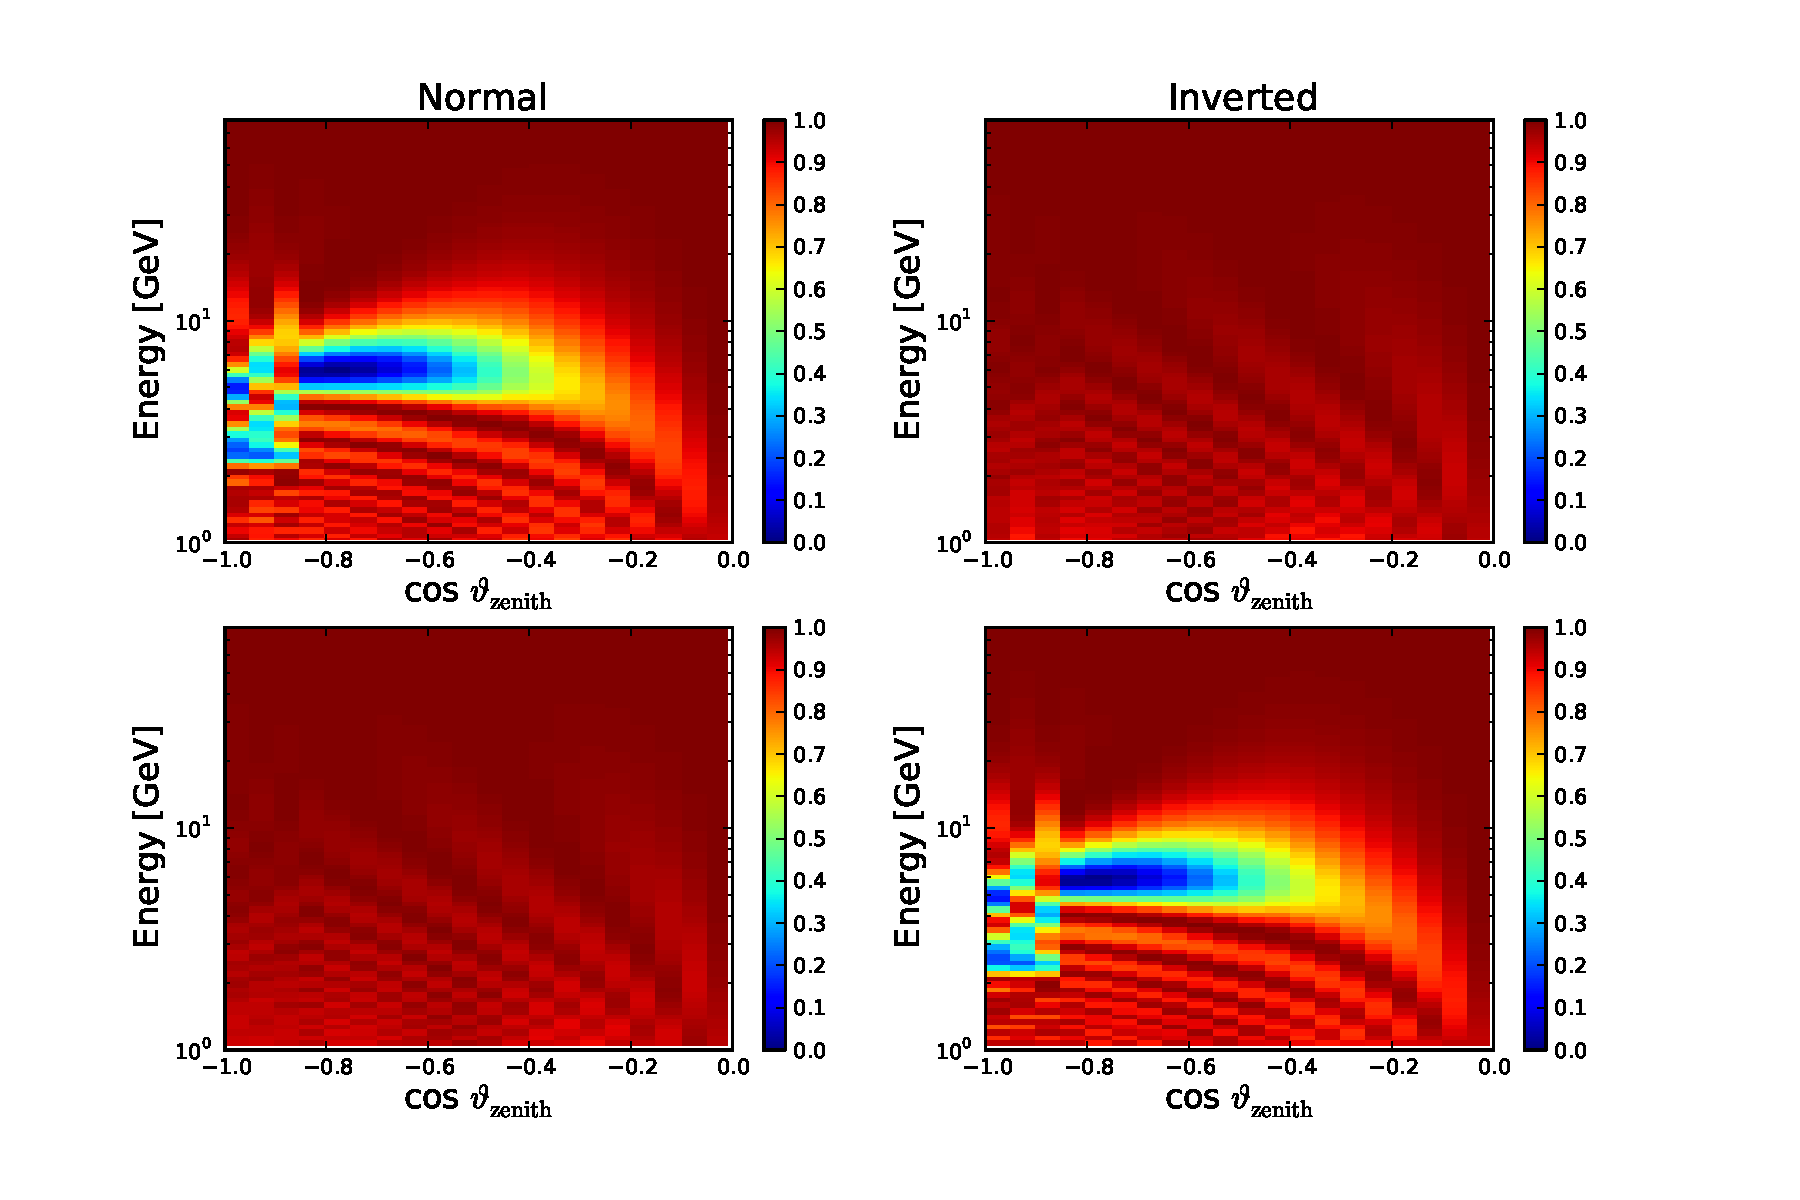
\includegraphics[width=0.95\textwidth]{osc_ds_nue_to_nue}
 \caption{Oscillation probabilities for $\nue \to \nue$ (top) and $\nuebar \to
          \nuebar$ (bottom) for normal and inverted hierarchy.}
\end{figure}


\begin{figure}[t!]
 \centering
 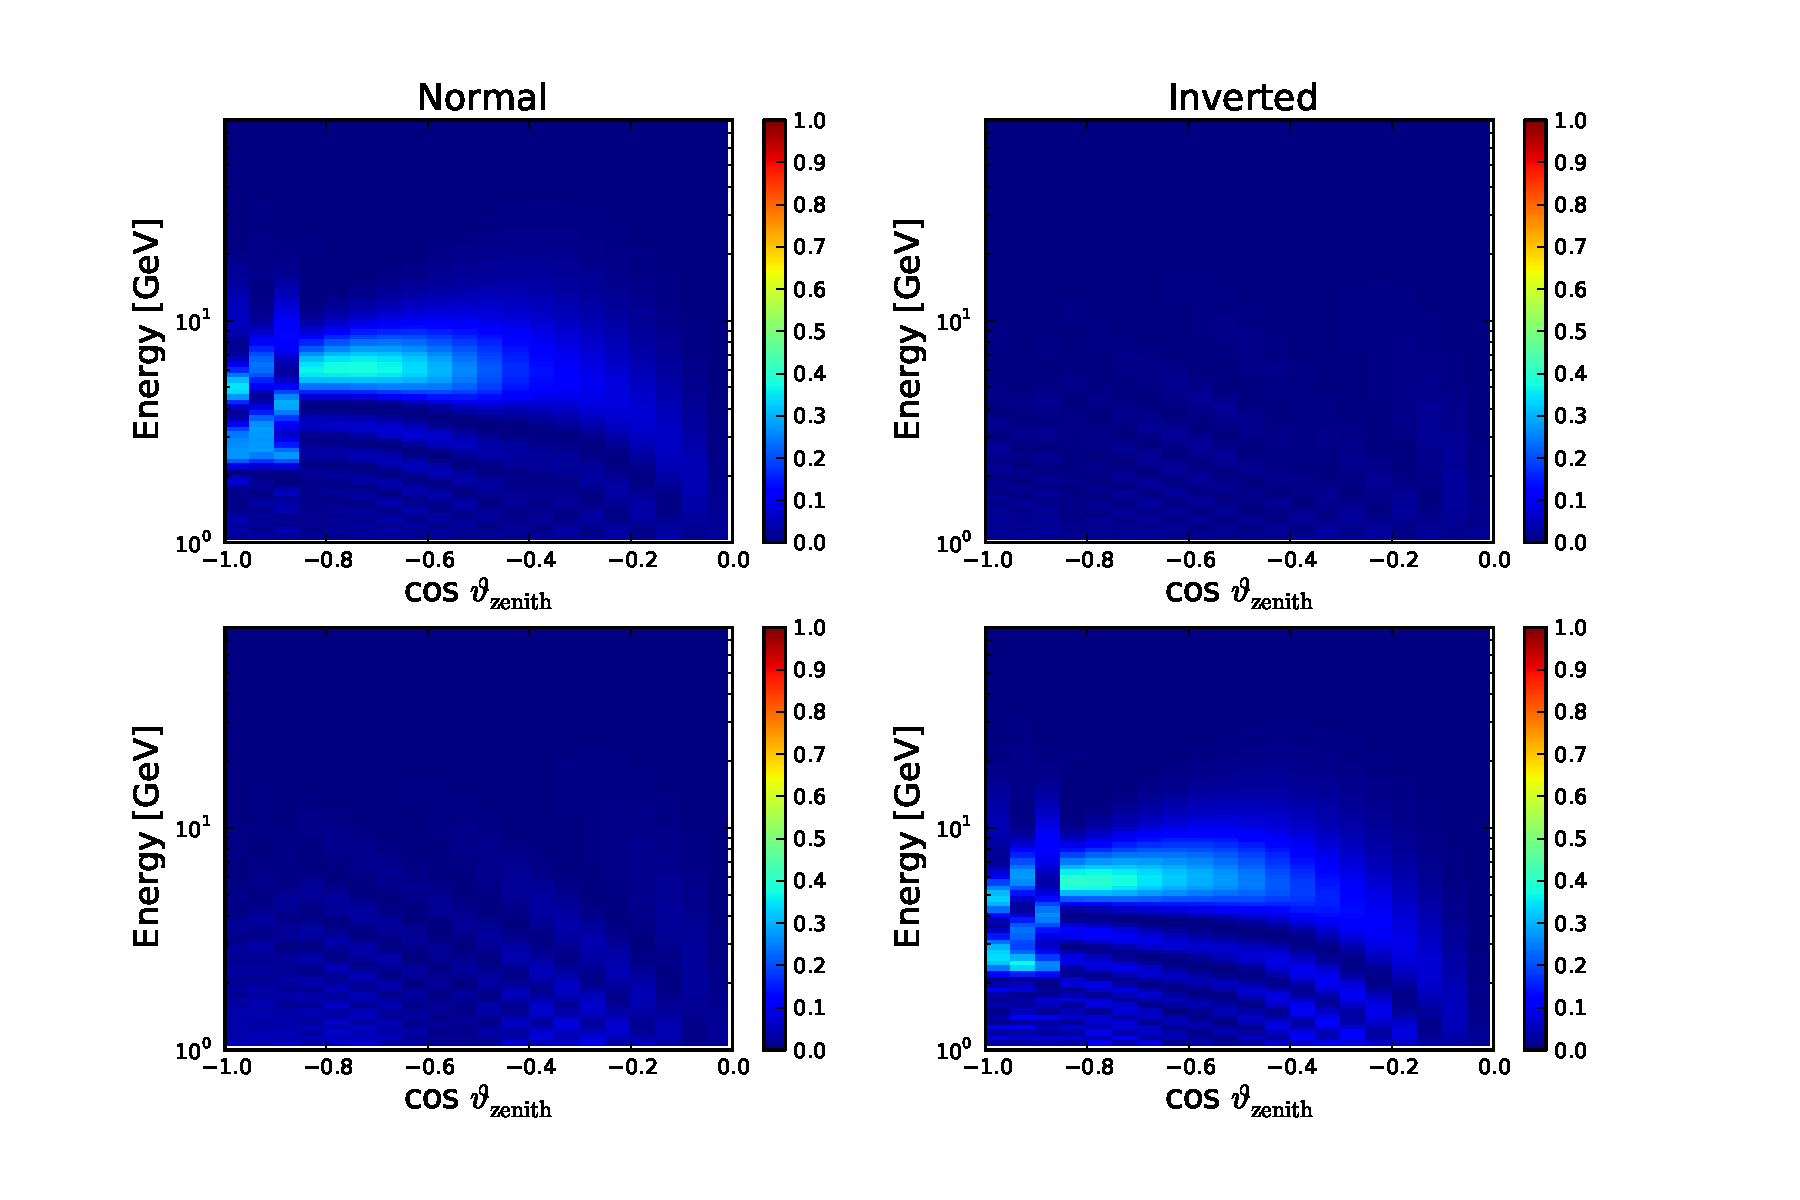
\includegraphics[width=0.95\textwidth]{osc_ds_nue_to_numu}
 \caption{Oscillation probabilities for $\nue \to \numu$ (top) and $\nuebar \to
          \numubar$ (bottom) for normal and inverted hierarchy.}
\end{figure}

\begin{figure}[b!]
 \centering
 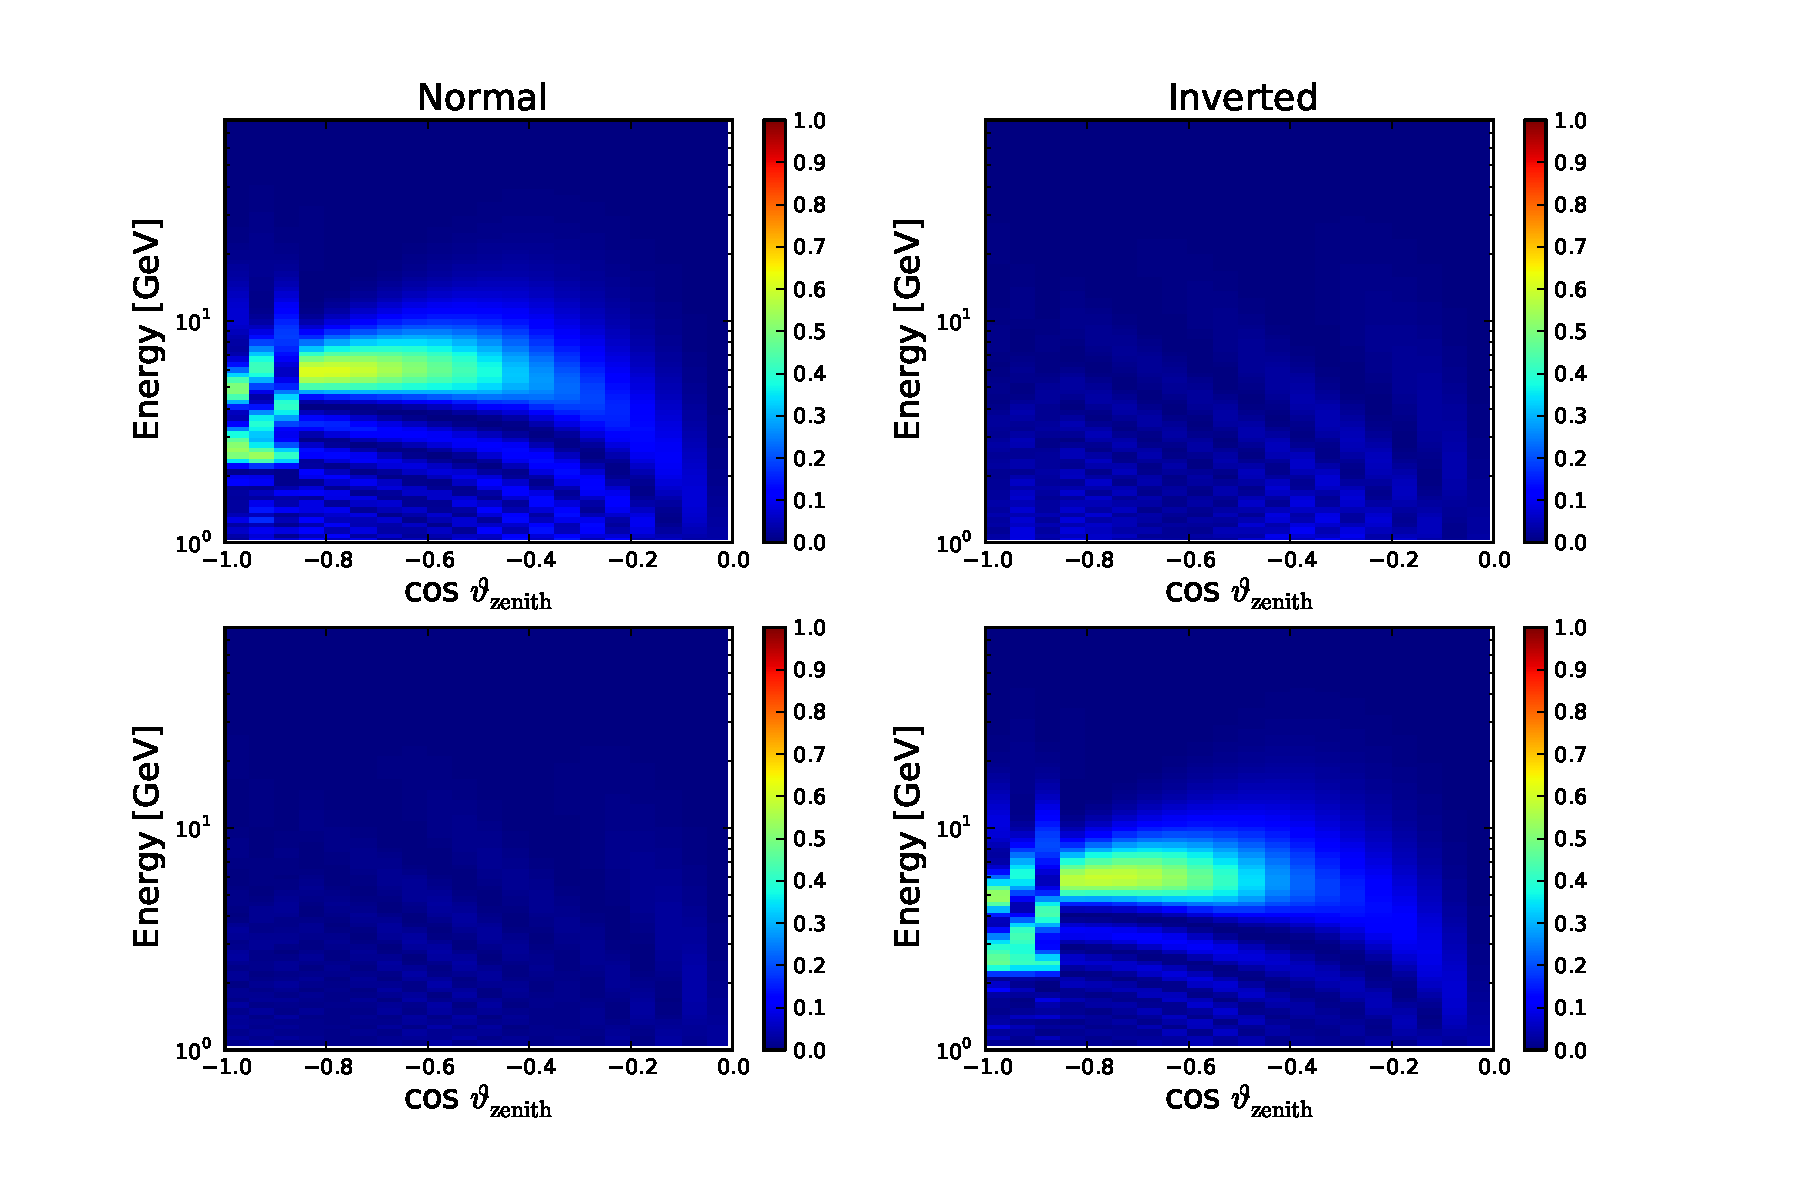
\includegraphics[width=0.95\textwidth]{osc_ds_nue_to_nutau}
 \caption{Oscillation probabilities for $\nue \to \nutau$ (top) and $\nuebar \to
          \nutaubar$ (bottom) for normal and inverted hierarchy.}
\end{figure}

\begin{figure}[t!]
 \centering
 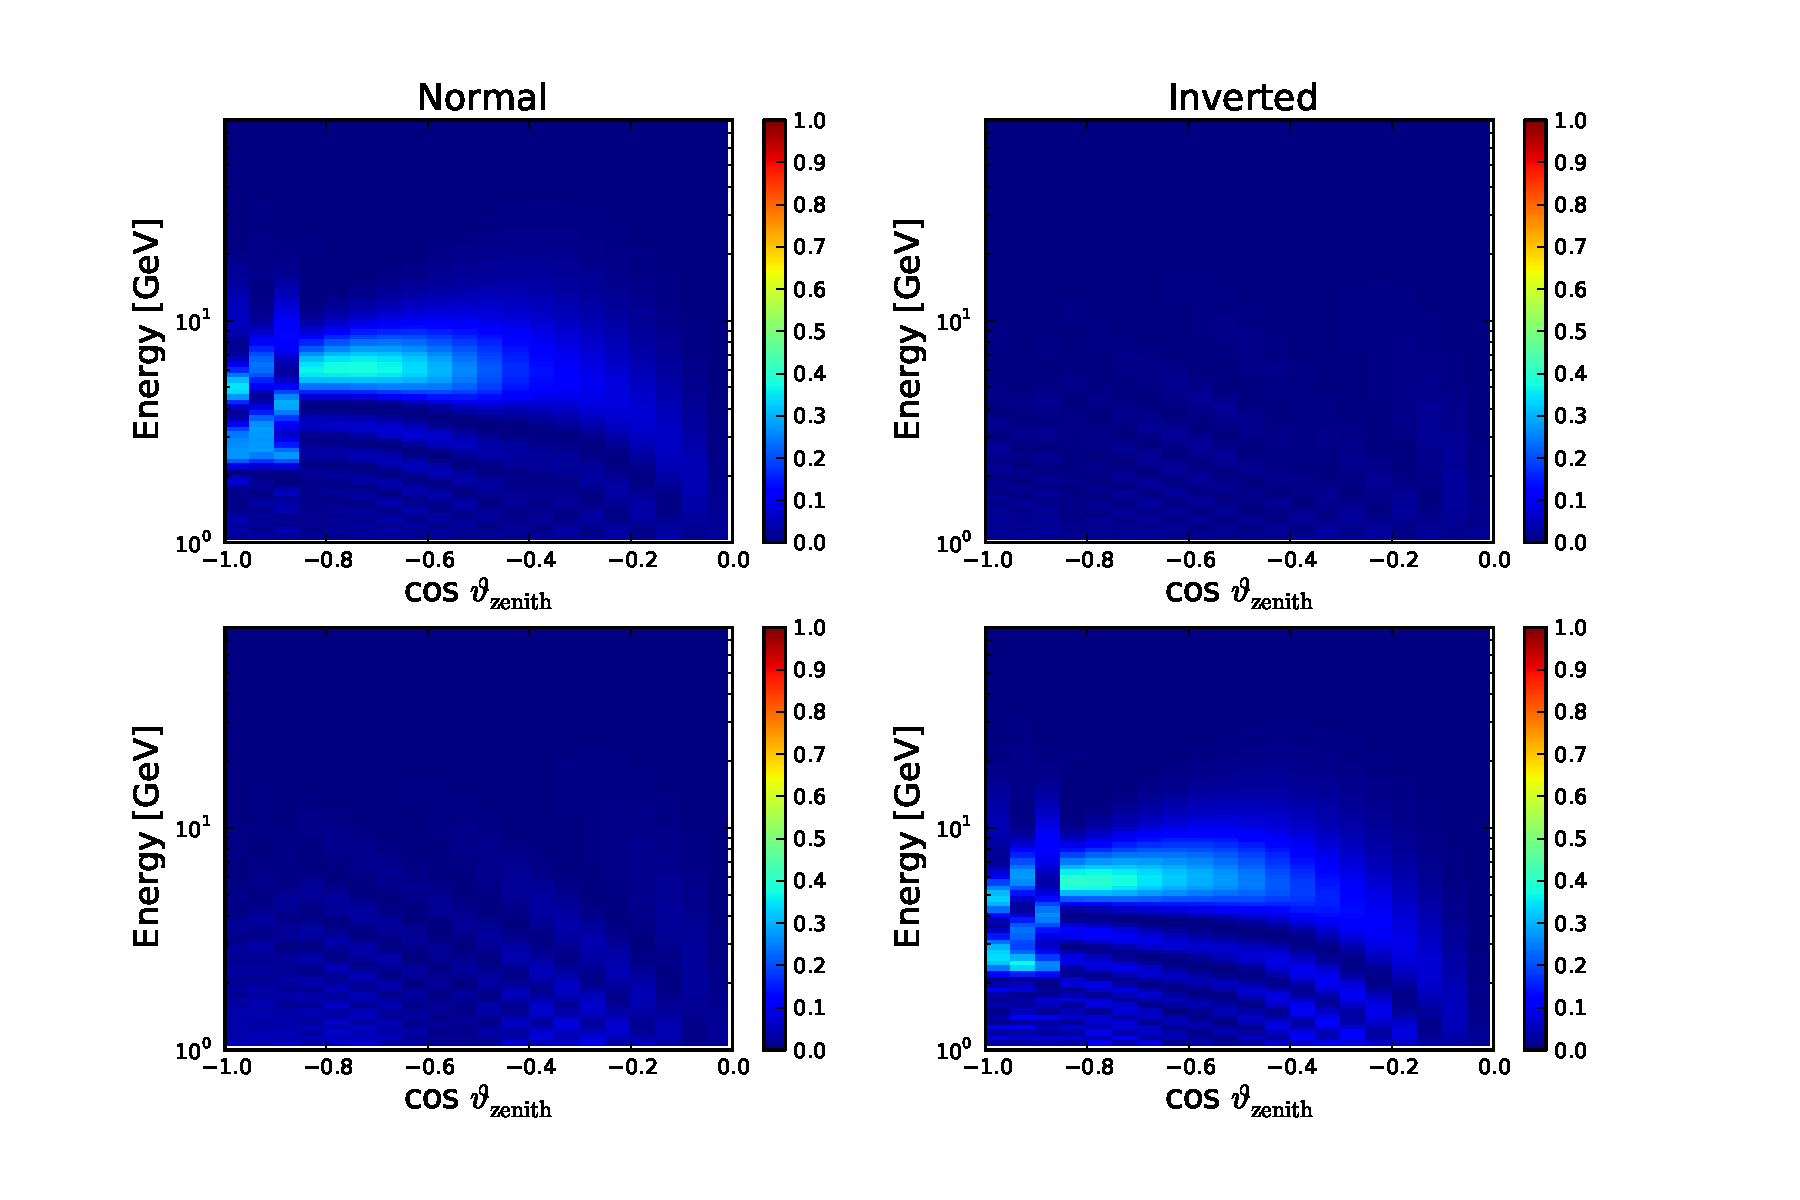
\includegraphics[width=0.95\textwidth]{osc_ds_numu_to_nue}
 \caption{Oscillation probabilities for $\numu \to \nue$ (top) and $\numubar \to
          \nuebar$ (bottom) for normal and inverted hierarchy.}
\end{figure}

\begin{figure}[b!]
 \centering
 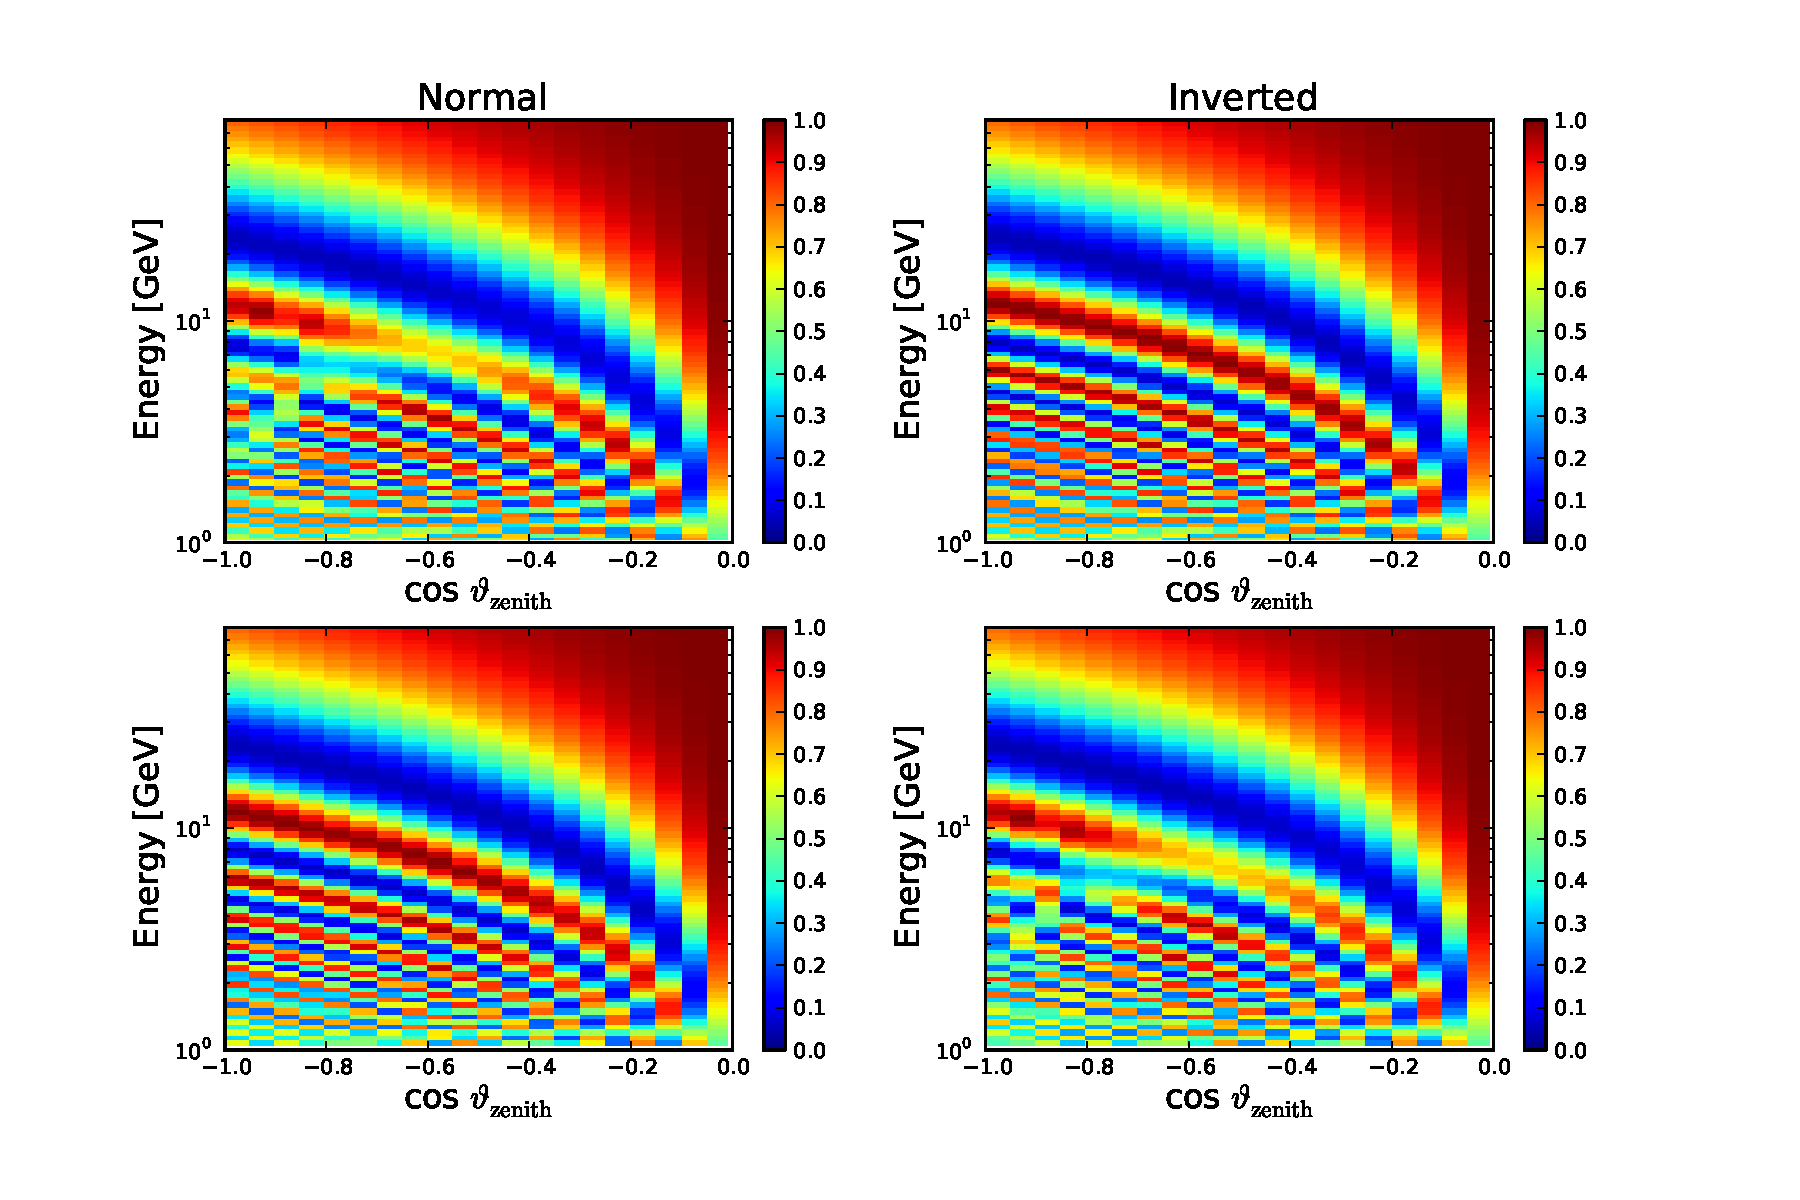
\includegraphics[width=0.95\textwidth]{osc_ds_numu_to_numu}
 \caption{Oscillation probabilities for $\numu \to \numu$ (top) and $\numubar
          \to \numubar$ (bottom) for normal and inverted hierarchy.}
\end{figure}


\begin{figure}[t!]
 \centering
 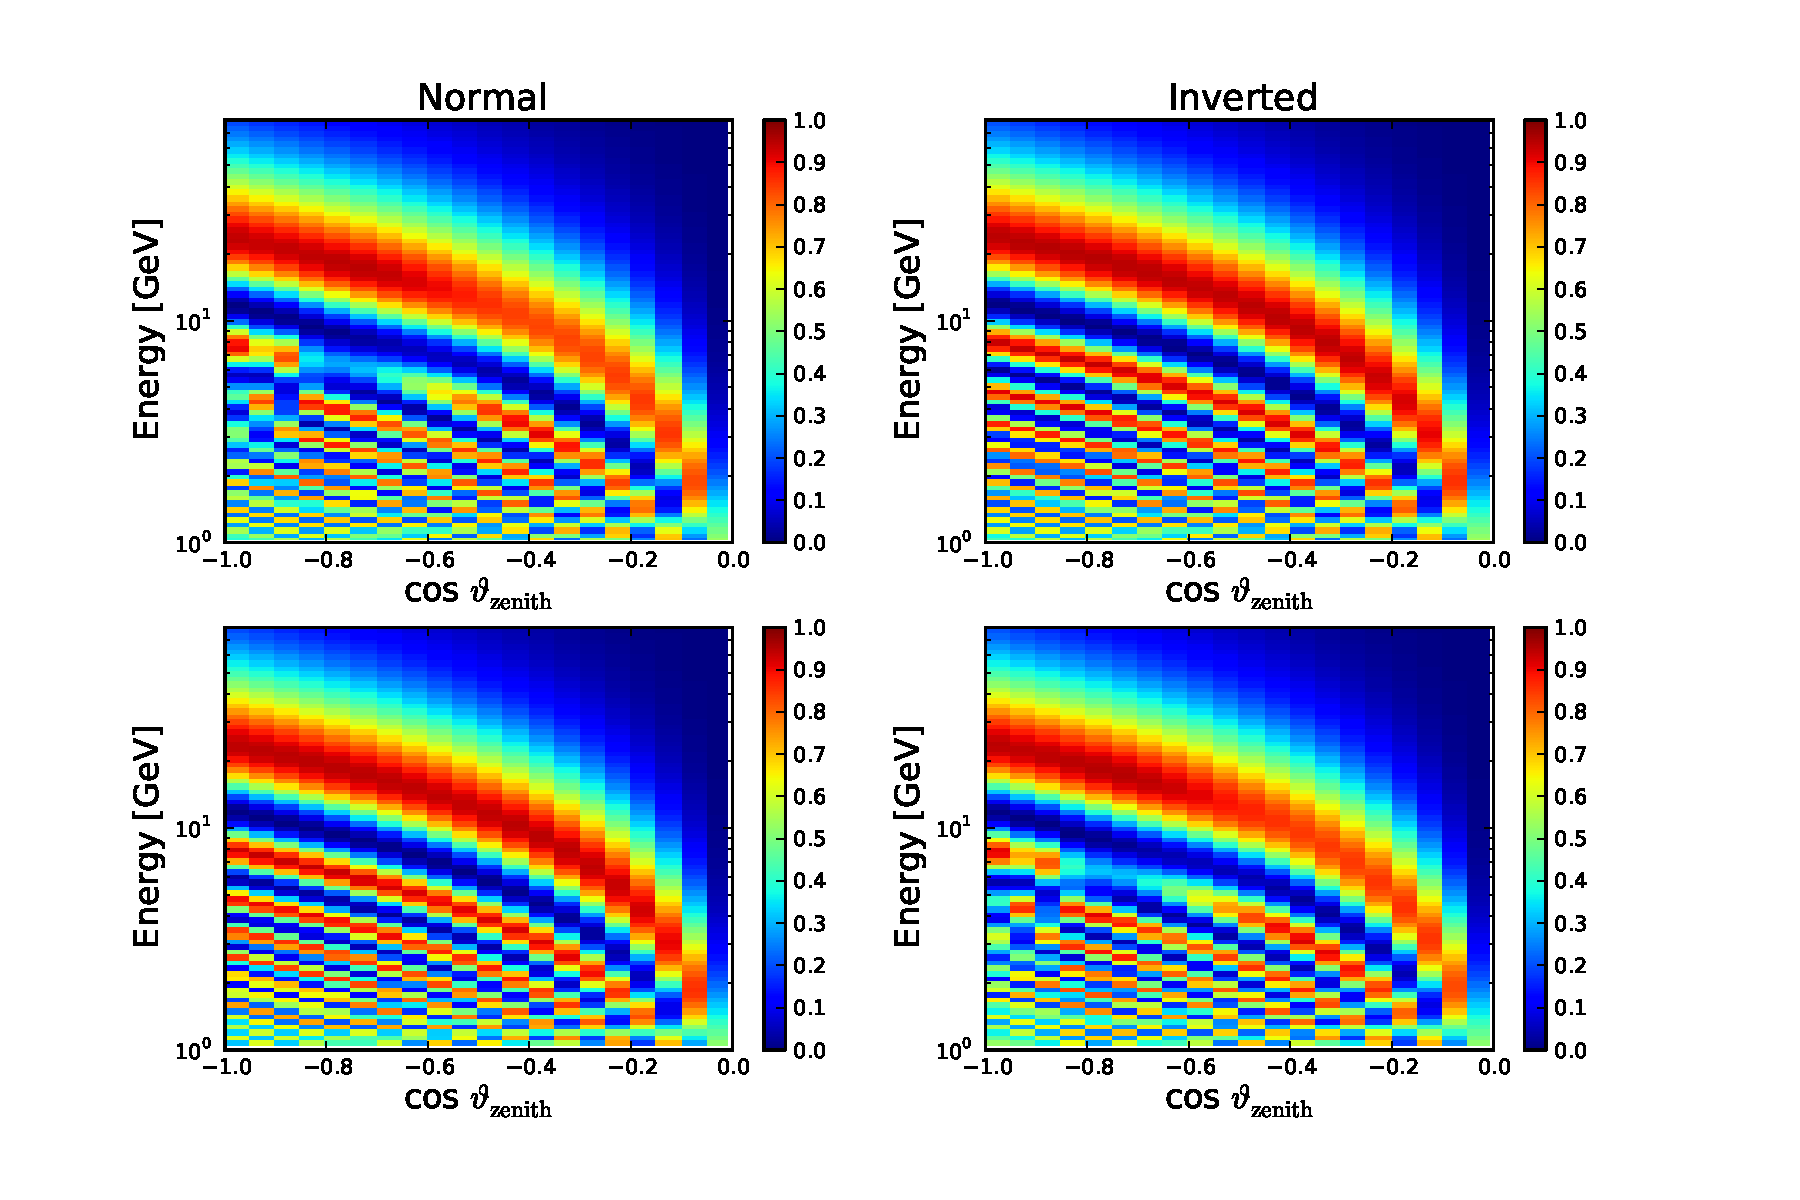
\includegraphics[width=0.95\textwidth]{osc_ds_numu_to_nutau}
 \caption{Oscillation probabilities for $\numu \to \nutau$ (top) and $\numubar
          \to \nutaubar$ (bottom) for normal and inverted hierarchy.}
\end{figure}

\clearpage
\section*{\refstepcounter{section}\thesection\quad Scanning the fiducial value
of \thet{23}}

\begin{figure}[b!]
 \centering
 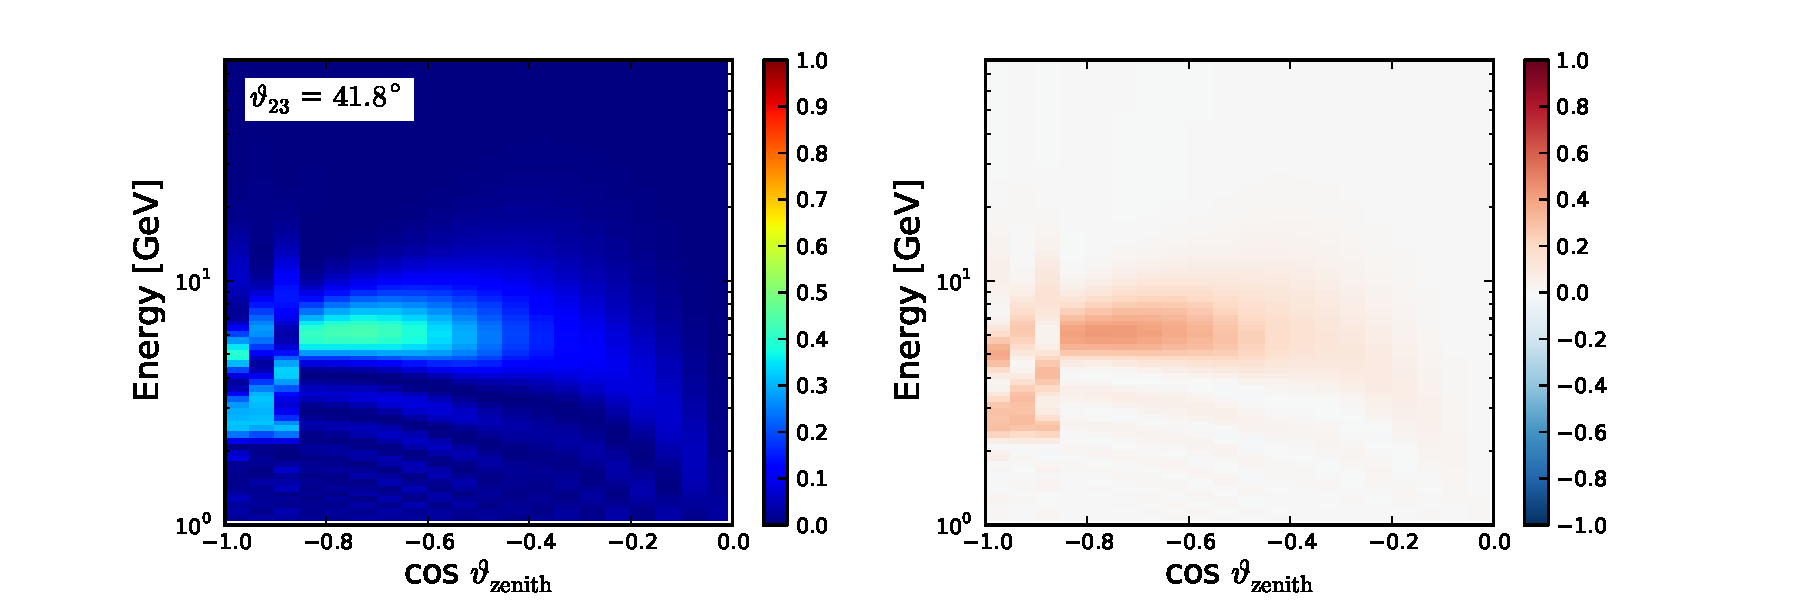
\includegraphics[width=0.9\linewidth]{P_NH_and_diff_numu_to_nue_th23_41deg}
 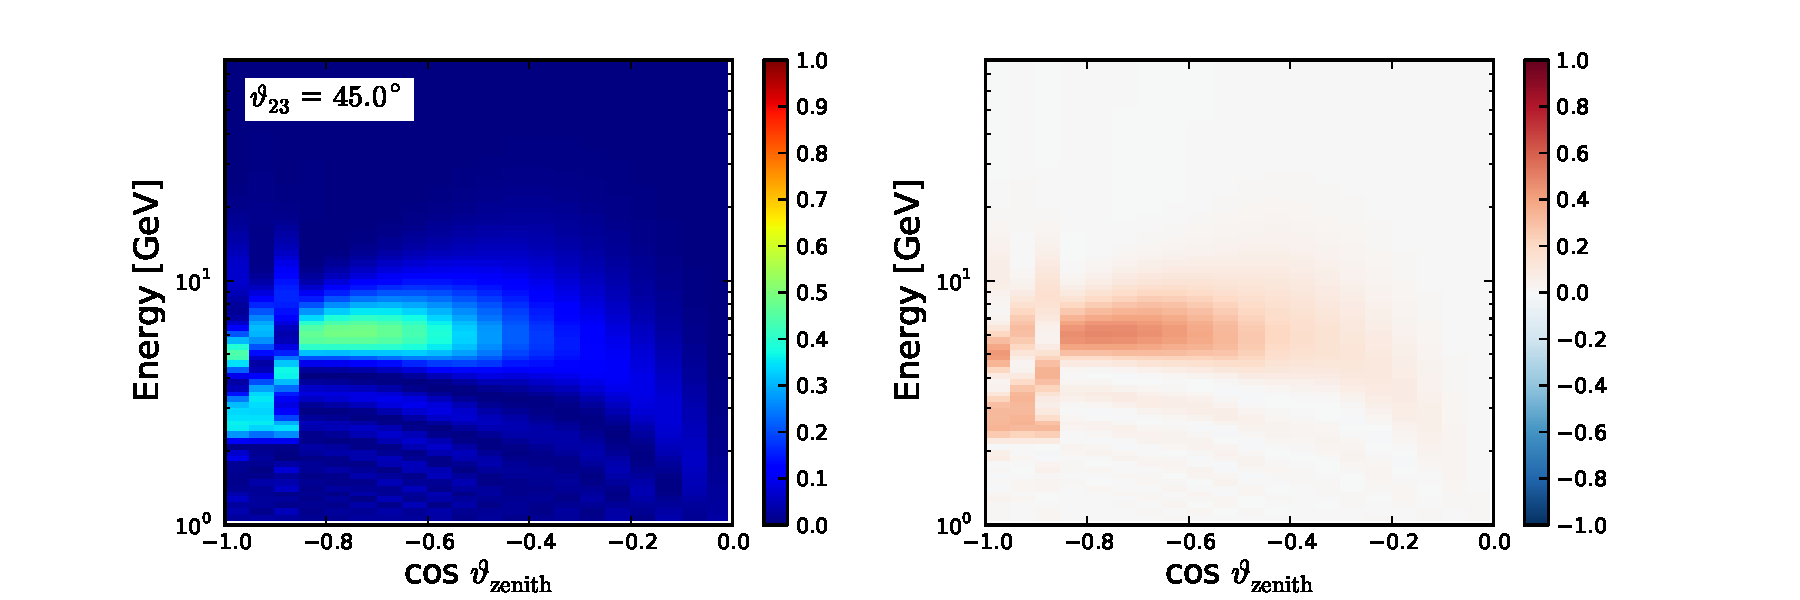
\includegraphics[width=0.9\linewidth]{P_NH_and_diff_numu_to_nue_th23_45deg}
 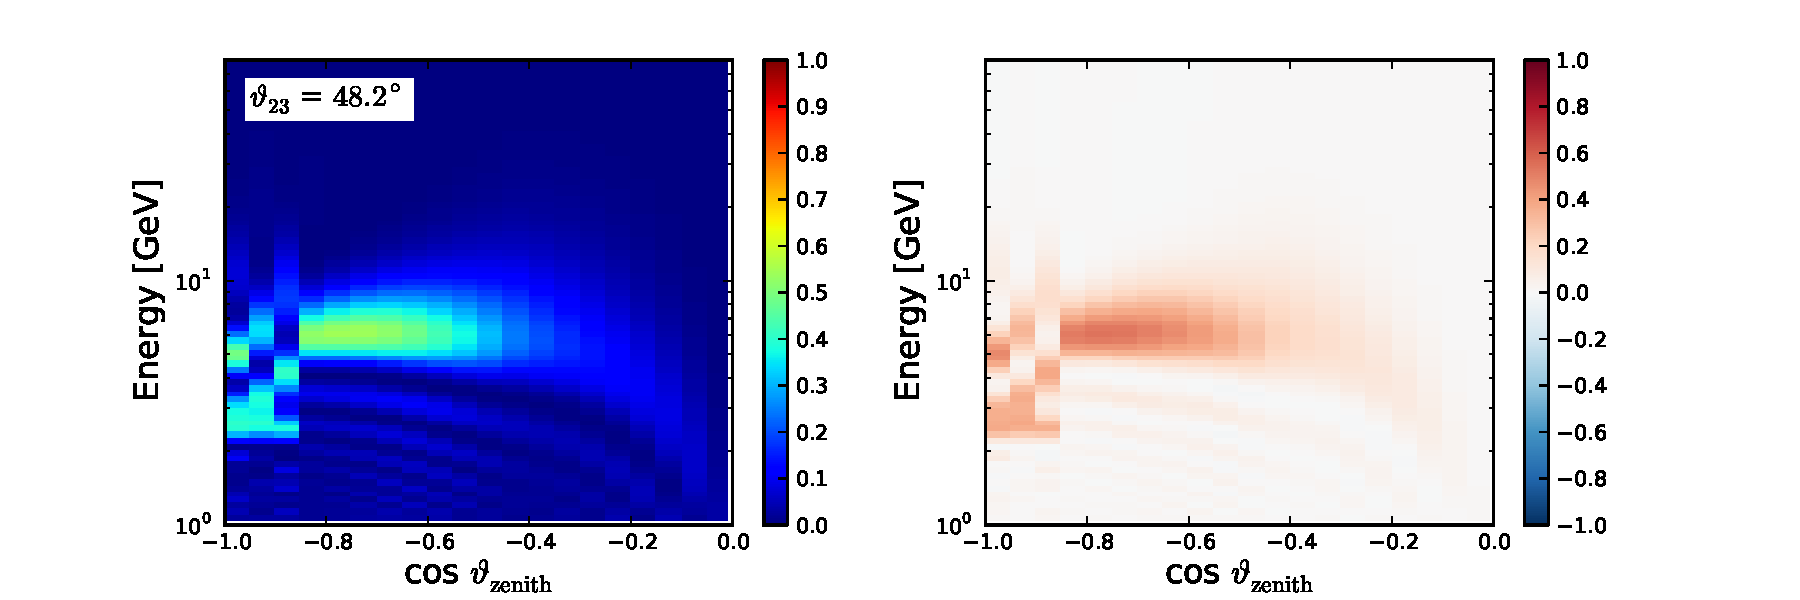
\includegraphics[width=0.9\linewidth]{P_NH_and_diff_numu_to_nue_th23_48deg}
 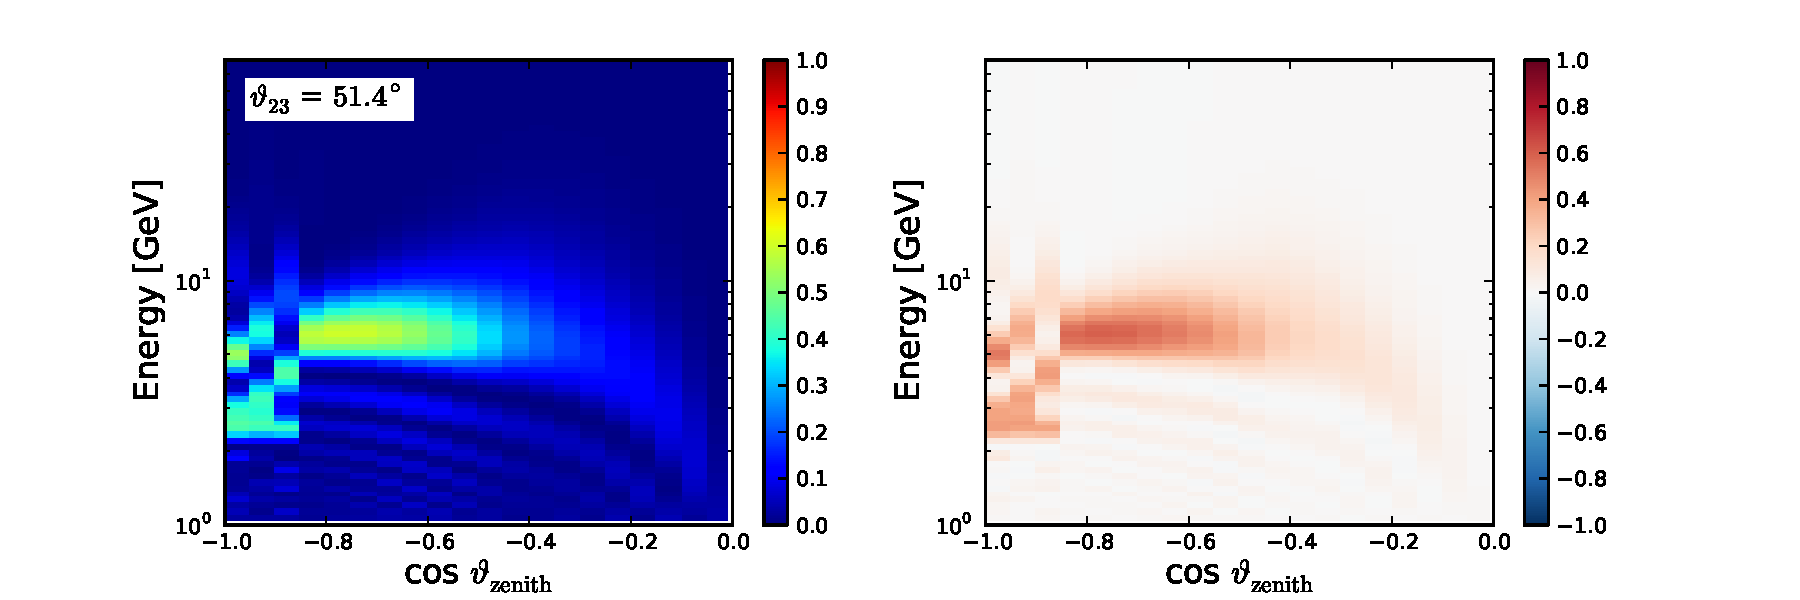
\includegraphics[width=0.9\linewidth]{P_NH_and_diff_numu_to_nue_th23_51deg}
 \caption{Probabilities for $\numu\to\nue$ oscillations in normal mass
  hierarchy (left column) and difference between normal and inverted hierarchy
  oscillation probabilities (right column) for different values of \thet{23} in
  both octants.}
 \label{fig:osc_probs_scan_th23}
\end{figure}


\chapter{Parametrisations of the Detector Resolutions}
\label{app:reco_params}

The full parametrisations of the reconstruction performances will be listed in
form of the actual \papa input. These are nested dictionaries giving the
resolutions in energy (\texttt{'e'}) and \coszen (\texttt{'coszen'}) for all
four interaction channels: \nue, \numu, and \nutau CC (\texttt{'nue'},
\texttt{'numu'}, and \texttt{'nutau'}, respectively) and \nux NC
(\texttt{'NC'}). For each of those the resolution is given by the five
parameters \texttt{'fraction'}, \texttt{'loc1'}, \texttt{'loc2'},
\texttt{'width1'}, and \texttt{'width2'}, corresponding to $f$, $\mu_1$,
$\mu_2$, $\sigma_1$ and $\sigma_2$ in (\ref{eqn:reco_param}).

The actual function definitions for the five parameters is then supplied as a
text string that can be interpreted as a python function by python's
\texttt{eval()} function. In those definitions, \texttt{'n'} is a shorthand
for the numpy library \cite{numpy} used for most of the numerical operations in
\papa.

\section*{\refstepcounter{section}\thesection\quad Baseline Settings}

\small{\VerbatimInput{figs/reco_param/reco_default.json}}

\section*{\refstepcounter{section}\label{app:reco_V15}\thesection\quad Geometry
V15 (Noiseless)}

\small{\VerbatimInput{figs/reco_param/reco_V15.json}}

\chapter{PID Functions}
\label{app:pid}

\section*{\refstepcounter{section}\thesection\quad Baseline Settings}

The particle identification is a binary decision, thus only the track
identification probabilities $P_{\mathrm{channel} \to \mathrm{track}}$ are
listed:
\begin{eqnarray}
 P_{\nue\to\mathrm{track}}(E) &=&
   0.192 \gauss{\log_{10}(E[\mathrm{GeV}])}{0.878}{0.404} + 0.0309 \\
 P_{\numu\to\mathrm{track}}(E) &=&
   \frac{0.687}{\stepfunc{\log_{10}(E[\mathrm{GeV}])}{0.683}{0.183}} + 0.0585 \\
 P_{\nutau\to\mathrm{track}}(E) &=&
   0.197 \gauss{\log_{10}(E[\mathrm{GeV}])}{1.28}{0.466} + 0.0732 \\
 P_{\nux\,\mathrm{NC}\to\mathrm{track}}(E) &=&
   0.171 \gauss{\log_{10}(E[\mathrm{GeV}])}{1.37}{0.483} + 0.0339
\end{eqnarray}
The cascade identification probabilities are given by $P_{\mathrm{channel} \to
\mathrm{cascade}} = 1 - P_{\mathrm{channel} \to \mathrm{track}}$.

\section*{\refstepcounter{section}\label{app:PID_threechannel}\thesection\quad 
High-Purity Event Classification}

\begin{figure}[h!]
 \centering
 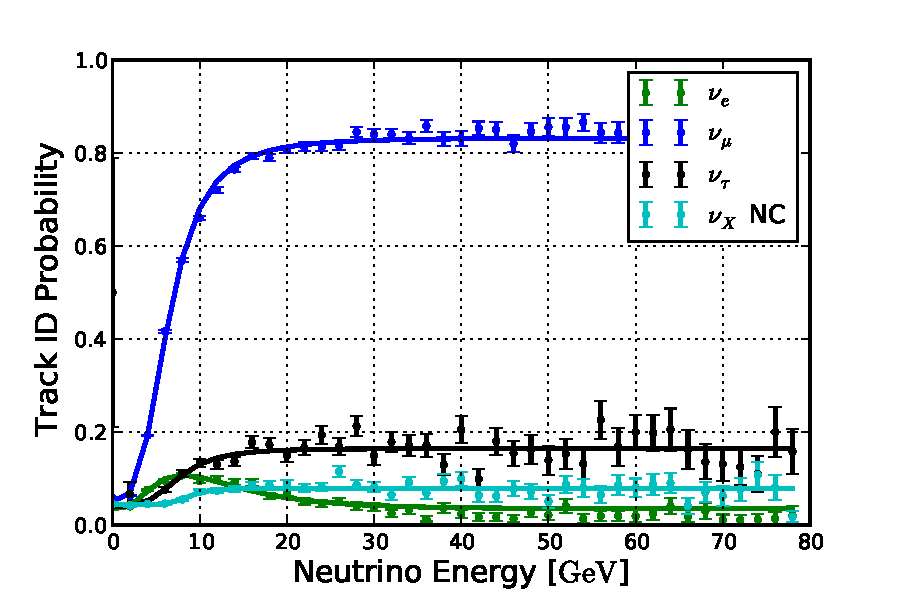
\includegraphics[width=0.495\linewidth]{PID_V15_trck}
 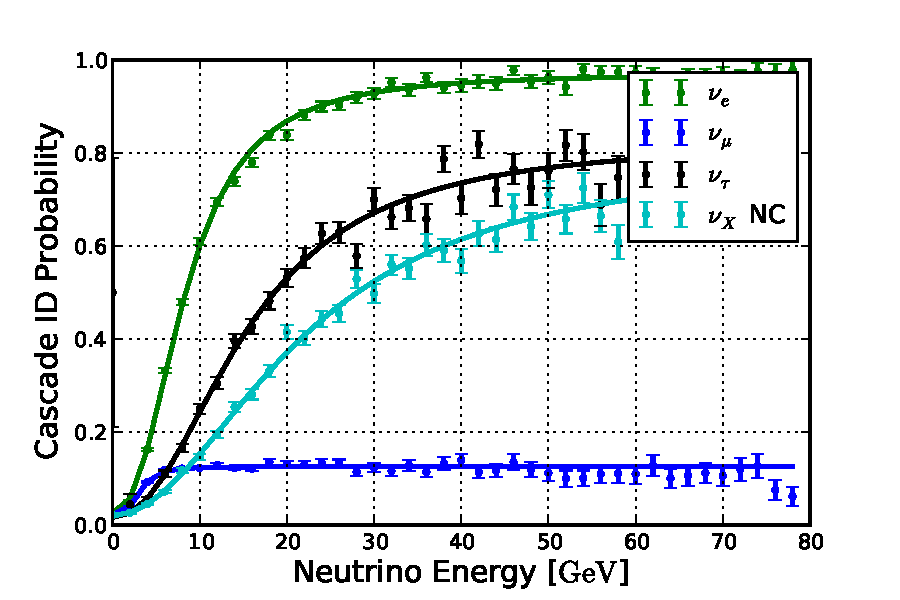
\includegraphics[width=0.495\linewidth]{PID_V15_cscd}
 \caption{Classification efficiencies for the high-purity track (left) and
          cascade (right) selections for PINGU V15, similar to
          Fig.~\ref{fig:PID}.}
 \label{fig:PID_threechannel}
\end{figure}

The particle identification is done by selecting high-purity track and cascade
samples, events ending up in neither sample are classified as ``unidentified'':
\begin{eqnarray}
 P_{\nue\to\mathrm{track}}(E) &=&
   0.0481 \gauss{\log_{10}(E[\mathrm{GeV}])}{0.904}{0.265} + 0.0350 \\
 P_{\nue\to\mathrm{cascade}}(E) &=&
   \frac{0.945}{\stepfunc{\log_{10}(E[\mathrm{GeV}])}{0.922}{0.180}} + 0.0264 \\
 P_{\numu\to\mathrm{track}}(E) &=&
   \frac{0.782}{\stepfunc{\log_{10}(E[\mathrm{GeV}])}{0.808}{0.135}} + 0.0507 \\
 P_{\numu\to\mathrm{cascade}}(E) &=&
   \frac{0.103}{\stepfunc{\log_{10}(E[\mathrm{GeV}])}{0.499}{0.127}} + 0.0223 \\
 P_{\nutau\to\mathrm{track}}(E) &=&
   \frac{0.125}{\stepfunc{\log_{10}(E[\mathrm{GeV}])}{0.882}{0.120}} + 0.0396 \\
 P_{\nutau\to\mathrm{cascade}}(E) &=&
   \frac{0.811}{\stepfunc{\log_{10}(E[\mathrm{GeV}])}{1.19}{0.200}} + 0.0163 \\
 P_{\nux\,\mathrm{NC}\to\mathrm{track}}(E) &=&
   \frac{0.0344}{\stepfunc{\log_{10}(E[\mathrm{GeV}])}{0.939}{0.0516}} + 0.0439
\\
 P_{\nux\,\mathrm{NC}\to\mathrm{cascade}}(E) &=&
   \frac{0.771}{\stepfunc{\log_{10}(E[\mathrm{GeV}])}{1.34}{0.216}} + 0.0202 
\end{eqnarray}
The fit of these functions to data is shown in Fig.~\ref{fig:PID_threechannel}.


\chapter{Full Error Listings}
\label{app:fisher_output}

Here the full error lists, similar to Tab.~\ref{tab:baseline_results}, for
various detector settings and sub-channels will be collected. These have
not been included in the main text for the sake of better readability. For a
description how to read the tables, refer to the explanations given for
Tab.~\ref{tab:baseline_results} in Sec.~\ref{sec:results_baseline}.

\section*{\refstepcounter{section}\label{app:fisher_baseline}\thesection\quad
Baseline Settings}

\begin{table}[h!]
 \caption{Same as Tab.~\ref{tab:baseline_results}, but for the track channel
  only}
 \begin{center}
  \small{\begin{tabular}{lrrrrrr} 
\toprule
Parameter & Impact [\%] & Best Fit & $\sigma^\mathrm{full}$ & $\sigma^\mathrm{stat}$ & $\sigma^\mathrm{syst}$ & Prior \\ 
\midrule
$h$ & 100.0 & \num{1.00e+00} & \num{7.47e-01} & \num{3.20e-01} & \num{6.75e-01} & free \\
$s_E$ & 8.4 & \num{1.00e+00} & \num{2.98e-02} & \num{8.36e-03} & \num{3.62e-02} & \num{5.00e-02} \\
$\Delta m^2_{31}$ [eV$^2$] & 7.2 & \num{2.46e-03} & \num{6.70e-05} & \num{1.93e-05} & \num{1.21e-04} & \num{8.00e-05} \\
$\vartheta_{23}$ [$^\circ$] & 5.9 & \num{3.86e+01} & \num{5.83e-01} & \num{3.55e-01} & \num{5.44e-01} & \num{1.32e+00} \\
$\vartheta_{13}$ [$^\circ$] & 3.6 & \num{8.93e+00} & \num{4.67e-01} & \num{9.47e-01} & \num{1.01e+01} & \num{4.68e-01} \\
$r_{\Phi,\,\nu_e-\nu_\mu}$ & 2.4 & \num{0.00e+00} & \num{3.61e-02} & \num{5.84e-03} & \num{5.17e-02} & \num{5.00e-02} \\
$\Delta_\mathrm{PID}$ [GeV] & 2.3 & \num{0.00e+00} & \num{3.82e-02} & \num{1.71e-02} & \num{3.43e-02} & \num{5.00e-01} \\
$s_\mathrm{PID}$ & 1.3 & \num{1.00e+00} & \num{3.04e-02} & \num{3.87e-03} & \num{3.01e-02} & free \\
$s_{A_\mathrm{eff}}$ [m$^2$/GeV] & 0.3 & \num{0.00e+00} & \num{4.13e-04} & \num{1.64e-04} & \num{3.79e-04} & free \\
$r_{A_\mathrm{eff},\,\nu-\bar\nu}$ & 0.2 & \num{0.00e+00} & \num{4.88e-02} & \num{9.29e-03} & \num{2.22e-01} & \num{5.00e-02} \\
\bottomrule 
\end{tabular}
}
 \end{center}
\end{table}

\begin{table}[h!]
 \caption{Same as Tab.~\ref{tab:baseline_results}, but for the cascade channel
  only}
 \begin{center}
  \small{\begin{tabular}{lrrrrrr} 
\toprule
Parameter & Impact [\%] & Best Fit & $\sigma^\mathrm{full}$ & $\sigma^\mathrm{stat}$ & $\sigma^\mathrm{syst}$ & Prior \\ 
\midrule
$h$ & 100.0 & \num{1.00e+00} & \num{5.17e-01} & \num{3.39e-01} & \num{3.91e-01} & free \\
$r_{\Phi,\,\nu_e-\nu_\mu}$ & 24.9 & \num{0.00e+00} & \num{2.44e-02} & \num{1.06e-02} & \num{2.58e-02} & \num{5.00e-02} \\
$\vartheta_{23}$ [$^\circ$] & 20.7 & \num{3.86e+01} & \num{1.05e+00} & \num{5.78e-01} & \num{1.61e+00} & \num{1.32e+00} \\
$\Delta_\mathrm{PID}$ [GeV] & 11.4 & \num{0.00e+00} & \num{1.53e-01} & \num{4.14e-02} & \num{1.55e-01} & \num{5.00e-01} \\
$s_{A_\mathrm{eff}}$ [m$^2$/GeV] & 4.5 & \num{0.00e+00} & \num{3.96e-04} & \num{1.85e-04} & \num{3.50e-04} & free \\
$r_{A_\mathrm{eff},\,\nu-\bar\nu}$ & 4.2 & \num{0.00e+00} & \num{4.91e-02} & \num{5.55e-03} & \num{2.60e-01} & \num{5.00e-02} \\
$\vartheta_{13}$ [$^\circ$] & 3.0 & \num{8.93e+00} & \num{4.66e-01} & \num{1.67e+00} & \num{5.53e+00} & \num{4.68e-01} \\
$s_E$ & 1.5 & \num{1.00e+00} & \num{3.14e-02} & \num{1.92e-02} & \num{3.55e-02} & \num{5.00e-02} \\
$\Delta m^2_{31}$ [eV$^2$] & 1.2 & \num{2.46e-03} & \num{6.73e-05} & \num{4.44e-05} & \num{1.16e-04} & \num{8.00e-05} \\
$n_{A_\mathrm{eff}}$ & 0.1 & \num{0.00e+00} & \num{2.29e-02} & \num{2.32e-03} & \num{2.29e-02} & \num{2.00e-01} \\
\bottomrule 
\end{tabular}
}
 \end{center}
\end{table}

\clearpage
\section*{\refstepcounter{section}\label{app:fisher_threechannel}
\thesection\quad High-Purity Event Classification}

\begin{table}[h!]
 \caption{Full error listings for the high-purity track channel, see
Sec.~\ref{sec:results_includeunkn}.}
 \begin{center}
  \small{\begin{tabular}{lrrrrrr} 
\toprule
Parameter & Impact [\%] & Best Fit & $\sigma^\mathrm{full}$ & $\sigma^\mathrm{stat}$ & $\sigma^\mathrm{syst}$ & Prior \\ 
\midrule
$h$ & 100.0 & \num{1.00e+00} & \num{1.10e+00} & \num{4.93e-01} & \num{9.86e-01} & free \\
$s_E$ & 21.3 & \num{1.00e+00} & \num{3.36e-02} & \num{1.31e-02} & \num{4.34e-02} & \num{5.00e-02} \\
$\Delta m^2_{31}$ [eV$^2$] & 10.7 & \num{2.46e-03} & \num{6.97e-05} & \num{3.03e-05} & \num{1.38e-04} & \num{8.00e-05} \\
$\vartheta_{23}$ [$^\circ$] & 6.1 & \num{3.86e+01} & \num{7.53e-01} & \num{5.50e-01} & \num{7.32e-01} & \num{1.32e+00} \\
$\Delta_\mathrm{PID}$ [GeV] & 3.6 & \num{0.00e+00} & \num{8.20e-02} & \num{3.98e-02} & \num{7.29e-02} & \num{5.00e-01} \\
$\vartheta_{13}$ [$^\circ$] & 1.7 & \num{8.93e+00} & \num{4.67e-01} & \num{1.46e+00} & \num{1.83e+01} & \num{4.68e-01} \\
$s_{A_\mathrm{eff}}$ [m$^2$/GeV] & 0.4 & \num{0.00e+00} & \num{6.16e-04} & \num{2.74e-04} & \num{5.52e-04} & free \\
$r_{\Phi,\,\nu_e-\nu_\mu}$ & 0.3 & \num{0.00e+00} & \num{4.37e-02} & \num{9.35e-03} & \num{8.96e-02} & \num{5.00e-02} \\
$s_\mathrm{PID}$ & 0.0 & \num{1.00e+00} & \num{2.05e-01} & \num{7.47e-03} & \num{2.05e-01} & free \\
$r_{A_\mathrm{eff},\,\nu-\bar\nu}$ & 0.0 & \num{0.00e+00} & \num{4.95e-02} & \num{1.78e-02} & \num{3.60e-01} & \num{5.00e-02} \\
$n_{A_\mathrm{eff}}$ & 0.0 & \num{0.00e+00} & \num{2.00e-01} & \num{7.47e-03} & NaN & \num{2.00e-01} \\
\bottomrule 
\end{tabular}
}
 \end{center}
\end{table}

\begin{table}[h!]
 \caption{Full error listings for the standard cascade channel (\ie cascades
are all events not identified as tracks), see
Sec.~\ref{sec:results_includeunkn}.}
 \label{tab:fisher_PID_cscd_nontracks}
 \begin{center}
  \small{\begin{tabular}{lrrrrrr} 
\toprule
Parameter & Impact [\%] & Best Fit & $\sigma^\mathrm{full}$ & $\sigma^\mathrm{stat}$ & $\sigma^\mathrm{syst}$ & Prior \\ 
\midrule
$h$ & 100.0 & \num{1.00e+00} & \num{7.30e-01} & \num{5.47e-01} & \num{4.83e-01} & free \\
$r_{\Phi,\,\nu_e-\nu_\mu}$ & 17.1 & \num{0.00e+00} & \num{3.12e-02} & \num{1.83e-02} & \num{3.54e-02} & \num{5.00e-02} \\
$\vartheta_{23}$ [$^\circ$] & 12.5 & \num{3.86e+01} & \num{1.26e+00} & \num{9.53e-01} & \num{4.03e+00} & \num{1.32e+00} \\
$s_{A_\mathrm{eff}}$ [m$^2$/GeV] & 7.7 & \num{0.00e+00} & \num{5.53e-04} & \num{3.37e-04} & \num{4.39e-04} & free \\
$n_{A_\mathrm{eff}}$ & 3.8 & \num{0.00e+00} & \num{2.33e-02} & \num{3.89e-03} & \num{2.32e-02} & \num{2.00e-01} \\
$\Delta_\mathrm{PID}$ [GeV] & 1.9 & \num{0.00e+00} & \num{1.78e-01} & \num{9.95e-02} & \num{1.62e-01} & \num{5.00e-01} \\
$r_{A_\mathrm{eff},\,\nu-\bar\nu}$ & 1.9 & \num{0.00e+00} & \num{4.96e-02} & \num{9.31e-03} & \num{3.74e-01} & \num{5.00e-02} \\
$\vartheta_{13}$ [$^\circ$] & 1.3 & \num{8.93e+00} & \num{4.67e-01} & \num{2.92e+00} & \num{8.26e+00} & \num{4.68e-01} \\
$s_E$ & 0.4 & \num{1.00e+00} & \num{3.64e-02} & \num{3.88e-02} & \num{3.65e-02} & \num{5.00e-02} \\
$\Delta m^2_{31}$ [eV$^2$] & 0.3 & \num{2.46e-03} & \num{7.03e-05} & \num{8.96e-05} & \num{1.17e-04} & \num{8.00e-05} \\
\bottomrule 
\end{tabular}
}
 \end{center}
\end{table}

% \begin{table}[h!]
%  \caption{Full error listings for the high-purity track channel, see
% Sec.~\ref{sec:results_includeunkn}.}
%  \begin{center}
%   \small{\begin{tabular}{lrrrrrr} 
\toprule
Parameter & Impact [\%] & Best Fit & $\sigma^\mathrm{full}$ & $\sigma^\mathrm{stat}$ & $\sigma^\mathrm{syst}$ & Prior \\ 
\midrule
$h$ & 100.0 & \num{1.00e+00} & \num{1.10e+00} & \num{4.93e-01} & \num{9.86e-01} & free \\
$s_E$ & 21.3 & \num{1.00e+00} & \num{3.36e-02} & \num{1.31e-02} & \num{4.34e-02} & \num{5.00e-02} \\
$\Delta m^2_{31}$ [eV$^2$] & 10.7 & \num{2.46e-03} & \num{6.97e-05} & \num{3.03e-05} & \num{1.38e-04} & \num{8.00e-05} \\
$\vartheta_{23}$ [$^\circ$] & 6.1 & \num{3.86e+01} & \num{7.52e-01} & \num{5.50e-01} & \num{7.29e-01} & \num{1.32e+00} \\
$\Delta_\mathrm{PID}$ [GeV] & 3.6 & \num{0.00e+00} & \num{8.09e-02} & \num{3.98e-02} & \num{7.16e-02} & \num{5.00e-01} \\
$\vartheta_{13}$ [$^\circ$] & 1.7 & \num{8.93e+00} & \num{4.67e-01} & \num{1.46e+00} & \num{1.83e+01} & \num{4.68e-01} \\
$s_{A_\mathrm{eff}}$ [m$^2$/GeV] & 0.4 & \num{0.00e+00} & \num{6.16e-04} & \num{2.74e-04} & \num{5.52e-04} & free \\
$r_{\Phi,\,\nu_e-\nu_\mu}$ & 0.3 & \num{0.00e+00} & \num{4.31e-02} & \num{9.35e-03} & \num{8.44e-02} & \num{5.00e-02} \\
$n_{A_\mathrm{eff}}$ & 0.2 & \num{0.00e+00} & \num{4.51e-02} & \num{7.47e-03} & \num{4.56e-02} & \num{2.00e-01} \\
$r_{A_\mathrm{eff},\,\nu-\bar\nu}$ & 0.0 & \num{0.00e+00} & \num{4.93e-02} & \num{1.78e-02} & \num{2.98e-01} & \num{5.00e-02} \\
\bottomrule 
\end{tabular}
}
%  \end{center}
% \end{table}


\begin{table}[h!]
 \caption{Full error listings for the high-purity cascade channel, see
Sec.~\ref{sec:results_includeunkn}.}
 \begin{center}
  \smaller{\begin{tabular}{lrrrrrr} 
\toprule
Parameter & Impact [\%] & Best Fit & $\sigma^\mathrm{full}$ & $\sigma^\mathrm{stat}$ & $\sigma^\mathrm{syst}$ & Prior \\ 
\midrule
$h$ & 100.0 & \num{1.00e+00} & \num{9.54e-01} & \num{6.35e-01} & \num{7.12e-01} & free \\
$\Delta_\mathrm{PID}$ [GeV] & 29.0 & \num{0.00e+00} & \num{9.77e-02} & \num{3.74e-02} & \num{9.24e-02} & \num{5.00e-01} \\
$r_{\Phi,\,\nu_e-\nu_\mu}$ & 21.4 & \num{0.00e+00} & \num{4.34e-02} & \num{4.50e-02} & \num{7.45e-02} & \num{5.00e-02} \\
$s_{A_\mathrm{eff}}$ [m$^2$/GeV] & 16.6 & \num{0.00e+00} & \num{1.06e-03} & \num{4.43e-04} & \num{9.64e-04} & free \\
$\vartheta_{23}$ [$^\circ$] & 2.8 & \num{3.86e+01} & \num{1.29e+00} & \num{3.02e+00} & \num{5.08e+00} & \num{1.32e+00} \\
$s_\mathrm{PID}$ & 1.2 & \num{1.00e+00} & \num{2.05e-01} & \num{9.07e-03} & \num{2.05e-01} & free \\
$s_E$ & 0.5 & \num{1.00e+00} & \num{4.12e-02} & \num{5.85e-02} & \num{4.30e-02} & \num{5.00e-02} \\
$\vartheta_{13}$ [$^\circ$] & 0.5 & \num{8.93e+00} & \num{4.67e-01} & \num{3.82e+00} & \num{1.20e+01} & \num{4.68e-01} \\
$r_{A_\mathrm{eff},\,\nu-\bar\nu}$ & 0.4 & \num{0.00e+00} & \num{5.00e-02} & \num{2.07e-02} & \num{1.41e+00} & \num{5.00e-02} \\
$\Delta m^2_{31}$ [eV$^2$] & 0.1 & \num{2.46e-03} & \num{7.38e-05} & \num{1.38e-04} & \num{1.32e-04} & \num{8.00e-05} \\
$n_{A_\mathrm{eff}}$ & 0.0 & \num{0.00e+00} & \num{2.00e-01} & \num{9.07e-03} & NaN & \num{2.00e-01} \\
\bottomrule 
\end{tabular}
}
 \end{center}
\end{table}

\begin{table}[h!]
 \caption{Full error listings for the sample of unidentified events, see
Sec.~\ref{sec:results_includeunkn}.}
 \begin{center}
  \smaller{\begin{tabular}{lrrrrrr} 
\toprule
Parameter & Impact [\%] & Best Fit & $\sigma^\mathrm{full}$ & $\sigma^\mathrm{stat}$ & $\sigma^\mathrm{syst}$ & Prior \\ 
\midrule
$h$ & 100.0 & \num{1.00e+00} & \num{1.13e+00} & \num{8.16e-01} & \num{7.80e-01} & free \\
$r_{\Phi,\,\nu_e-\nu_\mu}$ & 21.8 & \num{0.00e+00} & \num{4.14e-02} & \num{1.64e-02} & \num{7.21e-02} & \num{5.00e-02} \\
$n_{A_\mathrm{eff}}$ & 10.6 & \num{0.00e+00} & \num{2.49e-02} & \num{4.30e-03} & \num{2.47e-02} & \num{2.00e-01} \\
$s_E$ & 9.7 & \num{1.00e+00} & \num{4.22e-02} & \num{5.06e-02} & \num{6.06e-02} & \num{5.00e-02} \\
$s_\mathrm{PID}$ & 4.8 & \num{1.00e+00} & \num{6.42e-03} & \num{2.30e-03} & \num{6.00e-03} & free \\
$\Delta m^2_{31}$ [eV$^2$] & 4.1 & \num{2.46e-03} & \num{7.39e-05} & \num{1.15e-04} & \num{1.54e-04} & \num{8.00e-05} \\
$\Delta_\mathrm{PID}$ [GeV] & 3.9 & \num{0.00e+00} & \num{1.15e-01} & \num{4.72e-02} & \num{1.09e-01} & \num{5.00e-01} \\
$s_{A_\mathrm{eff}}$ [m$^2$/GeV] & 2.3 & \num{0.00e+00} & \num{2.32e-03} & \num{5.12e-04} & \num{2.26e-03} & free \\
$\vartheta_{23}$ [$^\circ$] & 1.8 & \num{3.86e+01} & \num{1.29e+00} & \num{9.74e-01} & \num{6.12e+00} & \num{1.32e+00} \\
$\vartheta_{13}$ [$^\circ$] & 0.6 & \num{8.93e+00} & \num{4.67e-01} & \num{3.74e+00} & \num{9.99e+00} & \num{4.68e-01} \\
$r_{A_\mathrm{eff},\,\nu-\bar\nu}$ & 0.5 & \num{0.00e+00} & \num{4.97e-02} & \num{1.04e-02} & \num{4.26e-01} & \num{5.00e-02} \\
\bottomrule 
\end{tabular}
}
 \end{center}
\end{table}

\enlargethispage{2cm}
\begin{table}[h!]
 \caption{Full error listings for the high-purity cascade channel combined with
the unidentified sample after Fisher matrix evaluation.}
 \label{tab:fisher_PID_cscd_twochan}
 \begin{center}
  \smaller{\begin{tabular}{lrrrrrr} 
\toprule
Parameter & Impact [\%] & Best Fit & $\sigma^\mathrm{full}$ & $\sigma^\mathrm{stat}$ & $\sigma^\mathrm{syst}$ & Prior \\ 
\midrule
$h$ & 100.0 & \num{1.00e+00} & \num{6.19e-01} & \num{5.01e-01} & \num{3.63e-01} & free \\
$\vartheta_{23}$ [$^\circ$] & 18.1 & \num{3.86e+01} & \num{1.20e+00} & \num{9.27e-01} & \num{2.74e+00} & \num{1.32e+00} \\
$r_{\Phi,\,\nu_e-\nu_\mu}$ & 6.7 & \num{0.00e+00} & \num{2.63e-02} & \num{1.54e-02} & \num{2.68e-02} & \num{5.00e-02} \\
$s_\mathrm{PID}$ & 4.3 & \num{1.00e+00} & \num{3.00e-03} & \num{2.23e-03} & \num{2.01e-03} & free \\
$s_{A_\mathrm{eff}}$ [m$^2$/GeV] & 3.3 & \num{0.00e+00} & \num{5.53e-04} & \num{3.35e-04} & \num{4.40e-04} & free \\
$r_{A_\mathrm{eff},\,\nu-\bar\nu}$ & 2.1 & \num{0.00e+00} & \num{4.94e-02} & \num{9.31e-03} & \num{3.31e-01} & \num{5.00e-02} \\
$\vartheta_{13}$ [$^\circ$] & 1.8 & \num{8.93e+00} & \num{4.67e-01} & \num{2.67e+00} & \num{7.62e+00} & \num{4.68e-01} \\
$n_{A_\mathrm{eff}}$ & 0.9 & \num{0.00e+00} & \num{2.19e-02} & \num{3.89e-03} & \num{2.16e-02} & \num{2.00e-01} \\
$s_E$ & 0.3 & \num{1.00e+00} & \num{3.63e-02} & \num{3.83e-02} & \num{3.64e-02} & \num{5.00e-02} \\
$\Delta_\mathrm{PID}$ [GeV] & 0.3 & \num{0.00e+00} & \num{3.37e-02} & \num{2.93e-02} & \num{1.69e-02} & \num{5.00e-01} \\
$\Delta m^2_{31}$ [eV$^2$] & 0.2 & \num{2.46e-03} & \num{7.02e-05} & \num{8.84e-05} & \num{1.17e-04} & \num{8.00e-05} \\
\bottomrule 
\end{tabular}
}
 \end{center}
\end{table}

\clearpage
\section*{\refstepcounter{section}\label{app:fisher_mDOM}
\thesection\quad PINGU equipped with mDOMs}

\begin{table}[h!]
 \caption{Full error listings for PINGU assuming reconstruction and particle
          identification as in geometry V15, \ie no module noise.}
 \label{tab:mDOM_comb}
 \begin{center}
  \smaller{\begin{tabular}{lrrrrrr} 
\toprule
Parameter & Impact [\%] & Best Fit & $\sigma^\mathrm{full}$ & $\sigma^\mathrm{stat}$ & $\sigma^\mathrm{syst}$ & Prior \\ 
\midrule
$h$ & 100.0 & \num{1.00e+00} & \num{3.33e-01} & \num{2.34e-01} & \num{2.37e-01} & free \\
$\vartheta_{23}$ [$^\circ$] & 12.5 & \num{3.86e+01} & \num{5.06e-01} & \num{2.81e-01} & \num{4.69e-01} & \num{1.32e+00} \\
$r_{\Phi,\,\nu_e-\nu_\mu}$ & 7.7 & \num{0.00e+00} & \num{9.32e-03} & \num{4.85e-03} & \num{8.15e-03} & \num{5.00e-02} \\
$r_{A_\mathrm{eff},\,\nu-\bar\nu}$ & 7.6 & \num{0.00e+00} & \num{4.78e-02} & \num{4.73e-03} & \num{1.62e-01} & \num{5.00e-02} \\
$\vartheta_{13}$ [$^\circ$] & 7.4 & \num{8.93e+00} & \num{4.64e-01} & \num{9.29e-01} & \num{3.46e+00} & \num{4.68e-01} \\
$n_{A_\mathrm{eff}}$ & 6.0 & \num{0.00e+00} & \num{1.93e-02} & \num{1.96e-03} & \num{1.93e-02} & \num{2.00e-01} \\
$\Delta m^2_{31}$ [eV$^2$] & 2.2 & \num{2.46e-03} & \num{6.59e-05} & \num{2.28e-05} & \num{1.14e-04} & \num{8.00e-05} \\
$\Delta_\mathrm{PID}$ [GeV] & 1.3 & \num{0.00e+00} & \num{2.31e-02} & \num{2.00e-02} & \num{1.16e-02} & \num{5.00e-01} \\
$s_E$ & 0.2 & \num{1.00e+00} & \num{2.88e-02} & \num{9.83e-03} & \num{3.39e-02} & \num{5.00e-02} \\
$s_{A_\mathrm{eff}}$ [m$^2$/GeV] & 0.1 & \num{0.00e+00} & \num{2.33e-04} & \num{1.47e-04} & \num{1.81e-04} & free \\
\bottomrule 
\end{tabular}
}
 \end{center}
\end{table}

\begin{table}[h!]
 \caption{Same as Tab.~\ref{tab:mDOM_comb}, but for the track channel
  only}
 \begin{center}
  \smaller{\begin{tabular}{lrrrrrr} 
\toprule
Parameter & Impact [\%] & Best Fit & $\sigma^\mathrm{full}$ & $\sigma^\mathrm{stat}$ & $\sigma^\mathrm{syst}$ & Prior \\ 
\midrule
$h$ & 100.0 & \num{1.00e+00} & \num{7.93e-01} & \num{3.65e-01} & \num{7.03e-01} & free \\
$s_E$ & 13.1 & \num{1.00e+00} & \num{3.14e-02} & \num{1.05e-02} & \num{3.91e-02} & \num{5.00e-02} \\
$\Delta m^2_{31}$ [eV$^2$] & 7.4 & \num{2.46e-03} & \num{6.80e-05} & \num{2.42e-05} & \num{1.26e-04} & \num{8.00e-05} \\
$\Delta_\mathrm{PID}$ [GeV] & 5.7 & \num{0.00e+00} & \num{5.21e-02} & \num{2.16e-02} & \num{4.78e-02} & \num{5.00e-01} \\
$\vartheta_{13}$ [$^\circ$] & 3.1 & \num{8.93e+00} & \num{4.67e-01} & \num{1.11e+00} & \num{1.08e+01} & \num{4.68e-01} \\
$\vartheta_{23}$ [$^\circ$] & 3.1 & \num{3.86e+01} & \num{5.85e-01} & \num{3.26e-01} & \num{5.65e-01} & \num{1.32e+00} \\
$n_{A_\mathrm{eff}}$ & 0.3 & \num{0.00e+00} & \num{3.58e-02} & \num{4.34e-03} & \num{3.61e-02} & \num{2.00e-01} \\
$r_{A_\mathrm{eff},\,\nu-\bar\nu}$ & 0.1 & \num{0.00e+00} & \num{4.88e-02} & \num{1.05e-02} & \num{2.28e-01} & \num{5.00e-02} \\
$r_{\Phi,\,\nu_e-\nu_\mu}$ & 0.0 & \num{0.00e+00} & \num{3.41e-02} & \num{5.59e-03} & \num{4.62e-02} & \num{5.00e-02} \\
$s_{A_\mathrm{eff}}$ [m$^2$/GeV] & 0.0 & \num{0.00e+00} & \num{4.99e-04} & \num{2.10e-04} & \num{4.53e-04} & free \\
\bottomrule 
\end{tabular}
}
 \end{center}
\end{table}

\enlargethispage{2cm}
\begin{table}[h!]
 \caption{Same as Tab.~\ref{tab:mDOM_comb}, but for the cascade channel
  only}
 \begin{center}
  \smaller{\begin{tabular}{lrrrrrr} 
\toprule
Parameter & Impact [\%] & Best Fit & $\sigma^\mathrm{full}$ & $\sigma^\mathrm{stat}$ & $\sigma^\mathrm{syst}$ & Prior \\ 
\midrule
$h$ & 100.0 & \num{1.00e+00} & \num{5.34e-01} & \num{3.04e-01} & \num{4.38e-01} & free \\
$r_{\Phi,\,\nu_e-\nu_\mu}$ & 43.4 & \num{0.00e+00} & \num{2.69e-02} & \num{9.78e-03} & \num{3.03e-02} & \num{5.00e-02} \\
$s_{A_\mathrm{eff}}$ [m$^2$/GeV] & 18.8 & \num{0.00e+00} & \num{4.92e-04} & \num{2.06e-04} & \num{4.46e-04} & free \\
$\vartheta_{23}$ [$^\circ$] & 10.4 & \num{3.86e+01} & \num{1.19e+00} & \num{5.56e-01} & \num{2.69e+00} & \num{1.32e+00} \\
$s_E$ & 6.7 & \num{1.00e+00} & \num{3.58e-02} & \num{2.83e-02} & \num{4.26e-02} & \num{5.00e-02} \\
$n_{A_\mathrm{eff}}$ & 5.1 & \num{0.00e+00} & \num{2.18e-02} & \num{2.20e-03} & \num{2.18e-02} & \num{2.00e-01} \\
$\Delta m^2_{31}$ [eV$^2$] & 2.5 & \num{2.46e-03} & \num{6.98e-05} & \num{6.61e-05} & \num{1.27e-04} & \num{8.00e-05} \\
$\Delta_\mathrm{PID}$ [GeV] & 2.5 & \num{0.00e+00} & \num{1.13e-01} & \num{5.25e-02} & \num{1.03e-01} & \num{5.00e-01} \\
$\vartheta_{13}$ [$^\circ$] & 2.3 & \num{8.93e+00} & \num{4.66e-01} & \num{1.71e+00} & \num{5.49e+00} & \num{4.68e-01} \\
$r_{A_\mathrm{eff},\,\nu-\bar\nu}$ & 2.2 & \num{0.00e+00} & \num{4.95e-02} & \num{5.29e-03} & \num{3.37e-01} & \num{5.00e-02} \\
\bottomrule 
\end{tabular}
}
 \end{center}
\end{table}


\backmatter
%------------------------------------------------------------------------------
% Declare bibliography, lists of figures and tables and
% acknowledgements as backmatter
% Chapter/section numbers are turned off

%------------------------------------------------------------------------------
% Include the following lines and comment out \printbibliography if
% you use BiBTeX for the bibliography.
% If you use biblatex package the files should de specified in the preamble.
%
% {\raggedright
%   \bibliographystyle{unsrt}
%   \bibliography{./thesis_refs,../refs/standard_refs-bibtex}
% }

%------------------------------------------------------------------------------
% Use biblatex for the bibliography
% Add bibliography to Table of Contents
\printbibliography[heading=bibintoc]

\listoffigures
\listoftables

%------------------------------------------------------------------------------
% Print the glossary and list of acronyms
% \printglossaries

%------------------------------------------------------------------------------
% You could instead add your acknowledgements here - don't forget to
% also add them to \includeonly above
% %------------------------------------------------------------------------------
\chapter*{Danksagung}
\label{sec:ack}
%------------------------------------------------------------------------------

\begin{otherlanguage}{ngerman}
Und das war es jetzt\dots\ Fehlt nur noch ein ganz gro\ss{}es Dankesch\"on an 
alle, ohne die diese Arbeit so nicht m\"oglich und die Zeit nicht so sch\"on 
gewesen w\"are.

Zuerst nat\"urlich an Marek Kowalski, der mir schon fr\"uh die Promotionsstelle 
zugesagt und mir sogar -- lang, lang ists her -- zu meiner Diplomarbeit schon 
ein paar n\"utzliche Tips gegeben hat. Auch sp\"ater war trotz vollen 
Terminplans und am Schluss auch gro\ss{}er Entfernung (fast) immer Zeit f\"ur 
ein paar hilfreiche Worte.
Danke auch an Norbert Wermes f\"ur die \"Ubernahme der Zweitkorrektur.

Dann der Bonner Doppel-Arbeitskreis. Sehr spannende Konstruktion, zwei doch 
ziemlich unterschiedliche Themen unter einem Dach. Erst mal vielen Dank an alle 
f\"ur die sch\"one Arbeitsatmosph\"are, den vielen leckeren Kuchen und die 
allmitt\"agliche Tee- und Kaffeepause. Besonderen Dank an meine flei\ss{}igen 
Korrekturleser Andreas, Markus, Alex und Marcel. Und weil Ruth auch was gelesen 
hat, sind meine Erg\"usse hoffentlich auch f\"ur Nicht-IceCuber verst\"andlich. 

Sebastian hat zwar nichts gelesen, aber trotzdem wohl am meisten beigetragen. 
Ob beim Programmieren, Debuggen, bei der Analyse oder bei Pr\"asentationen: 
Immer gab es hilfreiche Kommentare und Anregungen. Unter denen mag ich manchmal 
auch etwas gest\"ohnt haben, aber ein Faultier wie ich braucht den 
gelegentlichen Tritt in den Hintern. Und zur Belohnung ist er ja jetzt Prof 
im goldische Meenz.

Womit wir auch schon bei der Family w\"aren. Allen voran meine Schwestern 
Judith und Johanna, die zwar mittlerweile schon richtig erwachsen, aber 
trotzdem noch die lustigsten und liebsten Schwestern sind, die man haben kann. 
Au\ss{}erdem k\"onnen sie mich vermutlich beide unter den Tisch trinken -- 
Studenten halt. Dazu mein Onkel Mani, der tats\"achlich fast gleichzeitig mit 
mir aus Mainz gen Norden gezogen ist, allerdings nicht ganz so weit. Und meine 
Eltern: Danke f\"ur alles, trotz Allem.

Und zum Schluss noch einmal nach Bonn, zu den Polyphonikern: Ein toller Chor, 
nicht nur musikalisch, mit dem ich mich hier direkt heimisch gef\"uhlt habe. 
Dort hinzugehen, war eine der, wenn nicht die beste und wichtigste Entscheidung 
meines Lebens. 

Denn jetzt habe ich die beste Michi der Welt. Du hast mir das verr\"uckteste 
und sch\"onste Jahr meines Lebens geschenkt, dem noch bessere folgen werden. 
Und den besten Grund \"uberhaupt, endlich mal fertig zu werden. 

Das bin ich hiermit.


\end{otherlanguage}

%%% Local Variables: 
%%% mode: latex
%%% TeX-master: "../mythesis"
%%% End: 


%------------------------------------------------------------------------------
% CV needed when you submit your PhD thesis
%
% \definecolor{lightgray}{gray}{0.8}
\newcolumntype{L}{>{\raggedleft}p{0.15\textwidth}}
\newcolumntype{R}{p{0.8\textwidth}}
\newcommand\VRule{\color{lightgray}\vrule width 0.5pt}

\thispagestyle{empty}
\section*{Curriculum Vitae}

\subsection*{Personal Details}

\begin{tabular}{L!{\VRule}R}
Name & Lukas Schulte\\
Date of Birth &  21st June 1987\\
Email & schulte@physik.uni-bonn.de \\
Family status & Single
\end{tabular}

\subsection*{Education}

\begin{tabular}{L!{\VRule}R}
1997--2005 & Abitur, Theresianum, Mainz, Germany.\\
2005 & Internship at Deutsches Kunststoff-Institut, Darmstadt, Germany. \\
2005 & Internship at DESY, Hamburg, Germany. \\
2005--2011 & Diplom in Physics, Johannes-Gutenberg-Universität, Mainz,
Germany.\\
2011 & Schule für Astroteilchenphysik, Obertrubach-Bärnfels, Germany. \\
2011--2015 &  PhD in Physics, Rheinische Friedrich-Wilhelms-Universität, Bonn,
Germany. 
\end{tabular}

\subsection*{Professional Experience}

\begin{tabular}{L!{\VRule}R}
2005 & Internship at Deutsches Kunststoff-Institut, Darmstadt, Germany.
2005 & Internship at DESY, Hamburg, Germany.
2011--2015 & Doctoral work at the University of Bonn, Germany. \\
2013 & Poster at the International Cosmic Ray Conference, Rio de Janeiro,
Brazil. \\
2013 & Poster at the International Conference on Neutrino Physics and
Astrophysics, Boston, USA.
\end{tabular}

\subsection*{Languages}
\begin{tabular}{L!{\VRule}R}
German & Mother tongue \\
English & Fluent \\
Latin & Großes Latinum \\
Ancient Greek & Basics
\end{tabular}


\end{document}

%%% Local Variables:
%%% mode: latex
%%% TeX-master: t
%%% End:
